\documentclass[journal]{IEEEtran}

% ---------- Packages ----------
\usepackage{amsmath,amssymb,amsfonts,amsthm,mathtools}
\usepackage{graphicx}
\usepackage{booktabs}
\usepackage{cite}
\usepackage{url}
\usepackage{microtype}
\usepackage[caption=false,font=footnotesize]{subfig}
\usepackage{mathrsfs}
\usepackage{hyperref}
\hypersetup{hidelinks}
\usepackage{xcolor}
\usepackage[shortlabels]{enumitem}
\setlist[enumerate]{nosep,leftmargin=*}

\allowdisplaybreaks

% ---------- Theorem Environments ----------
\newtheorem{theorem}{Theorem}
\newtheorem{proposition}{Proposition}
\newtheorem{corollary}{Corollary}
\newtheorem{lemma}{Lemma}
\newtheorem{assumption}{Assumption}
\newtheorem{definition}{Definition}
\theoremstyle{remark}
\newtheorem{remark}{Remark}

% ---------- Macros ----------
\newcommand{\R}{\mathbb{R}}
\newcommand{\E}{\mathbb{E}}
\newcommand{\Prob}{\mathbb{P}}
\newcommand{\inner}[2]{\left\langle #1,#2\right\rangle}
\newcommand{\norm}[1]{\left\lVert #1\right\rVert}
\newcommand{\Id}{\mathsf{I}}
\newcommand{\diag}{\operatorname{diag}}
\newcommand{\sym}{\operatorname{sym}}
\newcommand{\skewop}{\operatorname{skew}}
\newcommand{\argmin}{\operatorname*{arg\,min}}
\newcommand{\cD}{\mathcal{D}}
\newcommand{\cN}{\mathcal{N}}

\newcommand{\bz}{\boldsymbol{z}}
\newcommand{\bu}{\boldsymbol{u}}
\newcommand{\bv}{\boldsymbol{v}}
\newcommand{\btheta}{\boldsymbol{\theta}}
\newcommand{\bpsi}{\boldsymbol{\psi}}
\newcommand{\bzero}{\boldsymbol{0}}
\newcommand{\bg}{\boldsymbol{g}}
\newcommand{\bH}{\boldsymbol{H}}
\newcommand{\bW}{\boldsymbol{W}}
\newcommand{\bS}{\boldsymbol{S}}
\newcommand{\bA}{\boldsymbol{A}}

\newcommand{\bF}{\boldsymbol{F}}
\newcommand{\bG}{\boldsymbol{G}}

\newcommand{\hatF}{\widehat{\boldsymbol{F}}}
\newcommand{\hatG}{\widehat{\boldsymbol{G}}}

\newcommand{\biasF}{\boldsymbol{b}^{F}}
\newcommand{\biasG}{\boldsymbol{b}^{G}}
\newcommand{\noiseF}{\boldsymbol{\xi}^{F}}
\newcommand{\noiseG}{\boldsymbol{\xi}^{G}}

\newcommand{\Vk}{\mathcal{V}}
\newcommand{\cE}{\mathcal{E}}
\newcommand{\cP}{\mathcal{P}}
\newcommand{\cC}{\mathcal{C}}
\newcommand{\cU}{\mathcal{U}}
\newcommand{\cG}{\mathcal{G}}
\newcommand{\cB}{\mathcal{B}}

% ---------- Title ----------
\title{Saddle-Field Policy Optimization for Zero-Sum Markov Games: Adaptive Lyapunov-Drift Control with Finite-Time Stationarity Guarantees}

\author{Jialin~Zhuang,~\IEEEmembership{Member,~IEEE,}
	and~Vincent~K.~N.~Lau,~\IEEEmembership{Fellow,~IEEE}%
	\thanks{J.~Zhuang and V.~K.~N.~Lau are with the Department of Electronic and Computer Engineering, The Hong Kong University of Science and Technology, Clear Water Bay, Hong Kong SAR, China (e-mail: jzhuangag@connect.ust.hk; eeknlau@ece.ust.hk).
		This work was supported by the Research Grants Council, Hong Kong, under Areas of Excellence Scheme Grants AoE/E-101/23-N and AoE/E-601/22-R.
		\textit{(Corresponding author: Vincent K. N. Lau.)}}
}

\begin{document}
	\maketitle
	
	% ============================================================
	\begin{abstract}
		Two-player zero-sum Markov games model robust reinforcement learning and competitive policy optimization.
		Their stochastic saddle fields can rotate near stationary points.
		We propose an online controller that assigns separate step sizes for field and curvature directions.
		A box-constrained quadratic program (QP) minimizes a model of the one-step change in a composite Lyapunov function $\Vk$, which combines weighted field energy and a regularized policy-space gap.
		A symmetric--antisymmetric Jacobian decomposition identifies when the curvature direction decreases field energy.
		For biased stochastic oracles, we prove an $O(1/K)$ bound on the time-average expected stationarity residual, where $K$ is the number of joint updates, plus a floor caused by oracle and local-model errors.
		A curvature-improvement condition lower-bounds the extra predicted decrease from the curvature step.
		If the field direction decreases $\Vk$ proportionally to its current value, $\E[\Vk]$ decreases geometrically to an error floor.
		A policy-space bound converts this result into bounds on the unregularized Nash gap and the maximizing player's worst-case-return loss.
		Experiments on normal-form, tabular, neural-policy, and trajectory-sampled games confirm the predicted geometry.
		Across these tasks, the controller attains consistently higher mean worst-case return and lower mean exploitability than the matched field-only ablation.
		On neural CyclicControl, it reduces final exploitability by $79.1\%$.
	\end{abstract}
	
	\begin{IEEEkeywords}
		Zero-sum Markov games, robust reinforcement learning, stochastic saddle fields, Lyapunov drift, adaptive step size.
	\end{IEEEkeywords}
	
	% ============================================================
	\section{Introduction}\label{sec:intro}
	% ============================================================
	\IEEEPARstart{T}{wo-player} zero-sum Markov games provide a standard framework
	for competitive policy optimization
	\cite{Shapley1953StochasticGames,Littman1994MarkovGames,Alacaoglu2022NACMG}.
	Robust reinforcement learning (RL) applies this framework to policies that must
	retain performance under model mismatch, disturbances, and adversarial
	perturbations
	\cite{SuttonBarto2018,MorimotoDoya2005RobustRL,Iyengar2005RobustDP,NilimElGhaoui2005}.
	Robust adversarial reinforcement learning (RARL) represents the task and
	disturbance policies as the maximizing and minimizing players
	\cite{Pinto2017RARL,Kamalaruban2020LangevinRARL}.
	
	Policy parameterization couples the two update blocks.
	Incompatible update scales may induce oscillatory or divergent recursions.
	Linear-quadratic analysis shows that alternating RARL updates without a
	stabilizing initialization can destabilize the closed-loop system, whereas a
	robustly stabilizing initialization and a double-loop update restore convergence guarantees
	\cite{ZhangHuBasar2020StabilityRARL}.
	
	\emph{Saddle-field viewpoint.}
	For differentiable maximizing- and minimizing-player policy parameters
	$\btheta$ and $\bpsi$, let $J(\btheta,\bpsi)$ denote the maximizing player's
	return and write $\bz\triangleq(\btheta,\bpsi)$.
	We express policy ascent and descent as the saddle field
	\begin{equation}\label{eq:Fdef}
		\bF(\bz)
		\triangleq
		\begin{bmatrix}
			-\nabla_{\btheta}J(\btheta,\bpsi)\\[0.2em]
			\phantom{-}\nabla_{\bpsi}J(\btheta,\bpsi)
		\end{bmatrix}.
	\end{equation}
	Here $\mathcal Z^{\star}\triangleq\{\bz:\bF(\bz)=\bzero\}$ is the
	first-order stationary set, and the Jacobian
	$\nabla\bF(\bz)$ is the derivative of $\bF$ with respect to $\bz$.
	Stochastic policy-gradient estimators provide noisy observations of this field
	and its Jacobian actions.
	
	Gradient descent--ascent (GDA) can rotate or diverge even on bilinear games.
	The proximal point method (PPM) and extragradient-type methods, including the
	classical extragradient method (EGM), Mirror-Prox, and policy extragradient,
	introduce stabilizing corrections
	\cite{Rockafellar1976PPM,Korpelevich1976Extragradient,Nemirovski2004MirrorProx,Mokhtari2020UnifiedEG,CenWeiChi2024FastPolicyEG}.
	For a scalar step size $s>0$, their representative updates are
	\begin{equation}\label{eq:classical_updates}
		\begin{aligned}
			\textnormal{GDA:}\quad
			\bz_{+}^{\rm GDA}&=\bz-s\bF(\bz),\\
			\textnormal{PPM:}\quad
			\bz_{+}^{\rm PPM}&=\bz-s\bF(\bz_{+}^{\rm PPM}),\\
			\textnormal{EGM:}\quad
			\widetilde{\bz}&=\bz-s\bF(\bz),\quad
			\bz_{+}^{\rm EGM}=\bz-s\bF(\widetilde{\bz}),
		\end{aligned}
	\end{equation}
	where $\widetilde{\bz}$ is the EGM extrapolation point.
	GDA is explicit, PPM is implicit, and EGM uses an extrapolated query to
	approximate the PPM correction.
	
	The local mechanism follows from the field energy and the curvature-induced
	direction
	\begin{equation}\label{eq:field_energy_curvature}
		\phi(\bz)\triangleq\tfrac12\norm{\bF(\bz)}^{2},
		\quad
		\bG(\bz)\triangleq\nabla\bF(\bz)\bF(\bz),
	\end{equation}
	where $\norm{\cdot}$ is the Euclidean norm.
	Because $\phi(\bz)\ge0$ and $\phi(\bz)=0$ exactly when
	$\bz\in\mathcal Z^{\star}$, field energy measures first-order stationarity.
	Proposition~\ref{prop:DTA} shows that PPM and EGM locally add
	$+s^{2}\bG$ to the GDA direction $-s\bF$.
	High-resolution ordinary differential equation (ODE) analysis also exposes
	curvature corrections that distinguish stable minimax updates from the basic
	field update \cite{Lu2022ODE}.
	Game decompositions separate $\nabla\bF$ into symmetric potential-like and
	antisymmetric Hamiltonian components
	\cite{Balduzzi2018Mechanics,Letcher2019DifferentiableGameMechanics}.
	Hamiltonian-gradient methods use $\nabla\bF^{\top}\bF$, whereas symplectic
	adjustments isolate antisymmetric coupling
	\cite{Mescheder2018GANConvergence,Loizou2020SHGD}.
	
	\emph{Two design questions.}
	Proposition~\ref{prop:DTA} fixes the step sizes of $-\bF$ and $+\bG$ to
	$(s,s^{2})$.
	A double-step stochastic extragradient method uses an extrapolation step size
	$\gamma_t>0$ and a final step size $\eta_t>0$, giving the local pair
	$(\eta_t,\eta_t\gamma_t)$
	\cite{Hsieh2020DSEG}.
	Adaptive Mirror-Prox selects a common geometry from past gradients
	\cite{Antonakopoulos2021AdaProx}; existing Lyapunov rules tune one step size
	\cite{Zhang2025AdaptivePolyak,Yuan2025StepSizeSDE}.
	These methods motivate two questions: When does $+\bG$ reduce field energy, and
	how should its step size be balanced with that of $-\bF$?
	
	We answer both questions with an online controller.
	It embeds $\phi$ and a regularized policy-space gap in a composite Lyapunov
	function $\Vk$.
	An exact symmetric--antisymmetric decomposition identifies when $+\bG$
	decreases $\phi$.
	A two-dimensional box-constrained quadratic program (QP) selects both step
	sizes by minimizing a local model of the one-step change in $\Vk$.
	
	\emph{Contributions.}
	The main contributions are as follows.
	\begin{itemize}[leftmargin=*,nosep]
		\item \textbf{Curvature geometry and adaptive step sizes.}
		An exact symmetric--antisymmetric condition characterizes curvature descent.
		A closed-form box QP selects both step sizes and gives no worse predicted
		change in $\Vk$ than feasible one-direction and fixed-coupling rules.
		\item \textbf{Finite-time stochastic guarantees.}
		For biased stochastic oracles, the time-average expected stationarity residual
		has an $O(1/K)$ transient, where $K$ is the number of joint updates, plus an
		explicit error floor.
		Under local field--Lyapunov alignment, $\E[\Vk]$ contracts geometrically, and
		Proposition~\ref{prop:performance_bridge} yields Nash-gap and worst-case-return
		bounds.
		\item \textbf{Mechanism and policy-game evidence.}
		Normal-form experiments verify the curvature geometry; population and
		trajectory-sampled Markov games show higher worst-case return and lower
		exploitability than the matched field-only ablation.
	\end{itemize}
	
	The rest of the paper is organized as follows.
	Section~\ref{sec:prelim} develops the saddle-field geometry.
	Sections~\ref{sec:drift} and~\ref{sec:conv} present the adaptive step-size rule
	and its stochastic analysis.
	Sections~\ref{sec:impl} and~\ref{sec:experiments} give the implementation and
	experiments.
	
	% ============================================================
	\section{Saddle-Field Formulation and the Geometry of the Curvature Direction}\label{sec:prelim}
	% ============================================================
	
	\subsection{Parameterized zero-sum Markov games as saddle fields}\label{subsec:formulation}
	
	We consider an infinite-horizon discounted two-player zero-sum Markov game with state space $\mathcal{S}$, maximizing-player action space $\mathcal{A}$, minimizing-player action space $\mathcal{B}$, transition kernel $P$, bounded reward $r$ to the maximizing player, discount factor $\alpha\in(0,1)$, and initial-state distribution $\rho$.
	Unless stated otherwise, all policy-space suprema and infima below are over stationary randomized Markov policies; for finite discounted zero-sum games this class contains optimal policies.
	For a maximizing-player policy $\pi$ and a minimizing-player policy $\nu$, the maximizing player's discounted return is
	\[
	J(\pi,\nu)
	\triangleq
	\E_{\rho,\pi,\nu}
	\!\left[
	\textstyle\sum_{t=0}^{\infty}\alpha^{t}r(s_{t},a_{t},b_{t})
	\right].
	\]
	Here $\E_{\rho,\pi,\nu}$ denotes expectation under the initial-state
	distribution and the two policies.
	The policy-space saddle objective is $\sup_{\pi}\inf_{\nu} J(\pi,\nu)$.
	Define the maximizing player's worst-case return, game value, and unregularized policy-space Nash gap by
	\begin{align}
		R_{\rm BR}(\pi)&\triangleq\inf_{\bar\nu}J(\pi,\bar\nu),
		&v^{\star}&\triangleq\sup_{\bar\pi}R_{\rm BR}(\bar\pi),\notag\\
		\operatorname{Gap}_{0}(\pi,\nu)
		&\triangleq
		\sup_{\bar\pi}J(\bar\pi,\nu)-\inf_{\bar\nu}J(\pi,\bar\nu).
		\label{eq:global_gap}
	\end{align}
	For finite action sets, define the discounted causal entropies
	\begin{align*}
		\mathsf H_{\alpha}^{\pi}(\pi,\nu)
		&\triangleq \E_{\rho,\pi,\nu}\!\left[\sum_{t\ge0}\alpha^t
		\bigl(-\log\pi(a_t\mid s_t)\bigr)\right],\\
		\mathsf H_{\alpha}^{\nu}(\pi,\nu)
		&\triangleq \E_{\rho,\pi,\nu}\!\left[\sum_{t\ge0}\alpha^t
		\bigl(-\log\nu(b_t\mid s_t)\bigr)\right],
	\end{align*}
	with the convention $0\log0=0$.
	For a regularization strength $\varepsilon\ge0$, define
	\begin{equation}\label{eq:entropic_return}
		J_{\varepsilon}(\pi,\nu)
		\triangleq J(\pi,\nu)
		+\varepsilon\mathsf H_{\alpha}^{\pi}(\pi,\nu)
		-\varepsilon\mathsf H_{\alpha}^{\nu}(\pi,\nu),
	\end{equation}
	with $\operatorname{Gap}_{\varepsilon}$ defined from $J_{\varepsilon}$ as in~\eqref{eq:global_gap}.
	
	\begin{proposition}[Policy-space performance bridge]\label{prop:performance_bridge}
		Suppose $\mathcal A$ and $\mathcal B$ are finite.
		For every policy pair
		$(\pi,\nu)$ and $\varepsilon\ge0$,
		\begin{equation}\label{eq:performance_bridge}
			\begin{aligned}
				0&\le v^{\star}-R_{\rm BR}(\pi)
				\le \operatorname{Gap}_{0}(\pi,\nu)\\
				&\le \operatorname{Gap}_{\varepsilon}(\pi,\nu)
				+\frac{\varepsilon\bigl(\log|\mathcal A|+\log|\mathcal B|\bigr)}{1-\alpha}.
			\end{aligned}
		\end{equation}
	\end{proposition}
	\begin{proof}
		The definition of $v^{\star}$ gives the first inequality, while
		$v^{\star}\le\sup_{\bar\pi}J(\bar\pi,\nu)$ gives the second.
		Write $A_\alpha=\log|\mathcal A|/(1-\alpha)$ and
		$B_\alpha=\log|\mathcal B|/(1-\alpha)$.
		The per-state entropy bound gives
		$0\le\mathsf H_\alpha^\pi\le A_\alpha$ and
		$0\le\mathsf H_\alpha^\nu\le B_\alpha$ for every policy pair, irrespective
		of the induced state distribution.
		Consequently, for fixed $\nu$,
		\[
		J(\bar\pi,\nu)
		=J_\varepsilon(\bar\pi,\nu)
		-\varepsilon\mathsf H_\alpha^\pi(\bar\pi,\nu)
		+\varepsilon\mathsf H_\alpha^\nu(\bar\pi,\nu)
		\le J_\varepsilon(\bar\pi,\nu)+\varepsilon B_\alpha,
		\]
		and hence $\sup_{\bar\pi}J(\bar\pi,\nu)\le
		\sup_{\bar\pi}J_\varepsilon(\bar\pi,\nu)+\varepsilon B_\alpha$.
		Likewise $J_\varepsilon(\pi,\bar\nu)\le
		J(\pi,\bar\nu)+\varepsilon A_\alpha$; consequently,
		$-\inf_{\bar\nu}J(\pi,\bar\nu)\le
		-\inf_{\bar\nu}J_\varepsilon(\pi,\bar\nu)+\varepsilon A_\alpha$.
		Adding the last two inequalities gives the final bound in~\eqref{eq:performance_bridge}.
	\end{proof}
	Thus a global entropy-regularized Nash gap controls the maximizing player's
	unregularized worst-case return up to a tunable entropy bias.
	The stationarity analysis below instead studies the local parameterized field.
	
	\begin{proposition}[Smooth finite-game performance component]\label{prop:smooth_entropy_gap}
		Suppose $\mathcal S,\mathcal A,\mathcal B$ are finite, the one-stage rewards are
		bounded, $\varepsilon>0$, and, on the parameter neighborhood under
		consideration, the current policies are $C^3$ with action probabilities
		bounded away from zero.
		Then the entropy-regularized best-response values against either current player,
		and hence $\operatorname{Gap}_\varepsilon$, are $C^3$ functions of the current
		policy parameters.
	\end{proposition}
	\begin{proof}
		Fix the minimizing-player policy.
		The maximizing player's soft Bellman value satisfies
		$v=T_\varepsilon(v;\bpsi)$, where each component of $T_\varepsilon$ is an
		$\varepsilon\log\sum\exp$ of the action values induced by $\nu_{\bpsi}$.
		Explicitly,
		\begin{align*}
			[T_\varepsilon(v;\bpsi)]_s
			&=\varepsilon\log\sum_a \exp\!\left(\frac{Q_\psi^v(s,a)}
			{\varepsilon}\right),\\
			Q_\psi^v(s,a)
			&\triangleq \bar r_\psi(s,a)
			+\alpha\sum_{s'}\bar P_\psi(s'|s,a)v_{s'} .
		\end{align*}
		Here $\mathcal H(p)\triangleq-\sum_i p_i\log p_i$ is the per-state Shannon
		entropy, $\bar P_\psi$ averages $P$ over $\nu_\psi$, and $\bar r_\psi$
		averages $r$ while including the opponent-entropy term
		$-\varepsilon\mathcal H(\nu_\psi(\cdot|s))$ from~\eqref{eq:entropic_return}.
		The map is $C^3$ in $(v,\bpsi)$, and its Jacobian with respect to $v$ is
		$\alpha P_{\pi_{\rm BR},\nu_{\bpsi}}$, a stochastic matrix scaled by $\alpha$.
		Thus $\|D_vT_\varepsilon\|_\infty\le\alpha<1$; therefore, the identity shift of
		$D_vT_\varepsilon$ is invertible by the Neumann series.
		The implicit-function theorem makes the unique soft fixed point $C^3$ in
		$\bpsi$.
		The minimizing player's soft-min Bellman equation has the same argument after replacing
		$\log\sum\exp$ by $-\log\sum\exp(-\cdot)$.
		Multiplication by $\rho$ gives the two regularized best-response values; their
		difference is $\operatorname{Gap}_\varepsilon$ and is therefore $C^3$.
	\end{proof}
	
	In large finite or continuous state spaces, exact dynamic programming is
	computationally prohibitive or requires solving a functional fixed-point
	problem. Modern methods therefore replace the policy-space problem by a
	parameterized one.
	The maximizing-player policy is represented by $\pi_{\btheta}(a\mid s)$ with $\btheta\in\R^{d_{\theta}}$, and the minimizing-player policy by $\nu_{\bpsi}(b\mid s)$ with $\bpsi\in\R^{d_{\psi}}$, giving
	\[
	\begin{aligned}
		J(\btheta,\bpsi)
		&\triangleq
		\E_{\rho,\pi_{\btheta},\nu_{\bpsi}}
		\!\left[
		\textstyle\sum_{t=0}^{\infty}\alpha^{t}r(s_{t},a_{t},b_{t})
		\right],\\
		&\hspace{3em}
		\max_{\btheta}\min_{\bpsi}J(\btheta,\bpsi).
	\end{aligned}
	\]
	
	In model-free training, stochastic policy-gradient estimators replace the exact
	gradients using trajectory-derived return, value, or advantage information
	\cite{Sutton2000PolicyGradient}.
	For the policy parameters above, $\bz\in\R^{d}$ in~\eqref{eq:Fdef}, where
	$d\triangleq d_{\theta}+d_{\psi}$.
	A point $\bz^{\star}\in\mathcal{Z}^{\star}$ is max-player ascent-stationary and
	min-player descent-stationary.
	Thus $\mathcal{Z}^{\star}$ is the first-order KKT set of the unconstrained
	parameterized objective.
	Corollary~\ref{cor:performance_contraction} connects the decrease in $\Vk$ to
	the policy-space Nash gap and worst-case return.
	
	The field $\bF$ in~\eqref{eq:Fdef} is the \emph{population target field}
	defined through exact policy gradients.
	Section~\ref{subsec:recursion_oracle_fixedpoint} models the implemented
	stochastic oracles and their estimation errors.
	
	We impose the following local regularity, used for the template expansion and
	the analysis of the one-step change in $\Vk$.
	
	\begin{assumption}[Local smoothness]\label{ass:smooth}
		There exists an open set $\cD\subset\R^{d}$ such that:
		\begin{enumerate}[(a)]
			\item all iterates and probing points used in the analysis lie in $\cD$;
			\item $J:\R^{d}\to\R$ is $C^{4}$ on $\cD$;
			\item all derivatives of $J$ up to order four are bounded on $\cD$.
		\end{enumerate}
	\end{assumption}
	
	Conditions (b)--(c) imply $\bF\in C^{3}(\cD;\R^{d})$, the regularity used throughout; condition (a) is an admissibility requirement enforced in implementations by the safeguards of Section~\ref{sec:impl}.
	
	\subsection{Classical templates and the curvature-induced direction}\label{subsec:expansions}
	
	For a smooth saddle field, the goal is to find $\bz^{\star}$ with $\bF(\bz^{\star})=\bzero$.
	Eq.~\eqref{eq:classical_updates} defines the GDA, PPM, and EGM updates used below.
	Proposition~\ref{prop:DTA} makes their local second-order relation precise.
	
	The stabilizing mechanism is visible on the bilinear max--min saddle
	$L(x,y)=-xy$, which is consistent with the sign convention in~\eqref{eq:Fdef}
	and has field $\bF=J_{0}\bz$, where
	\[
		J_{0}
		\triangleq
		\begin{bmatrix}
			0&1\\
			-1&0
		\end{bmatrix}.
	\]
	This matrix satisfies $J_{0}^{2}=-\Id_{2}$, where $\Id_n$ denotes the
	$n\times n$ identity.
	GDA has eigenvalue modulus
	$\sqrt{1+s^{2}}>1$ and spirals outward; PPM contracts for every $s>0$, while
	EGM contracts for $0<s<1$ (is neutral at $s=1$ and expansive for $s>1$).
	Recall $\phi$ and $\bG$ from~\eqref{eq:field_energy_curvature}.
	Below, $\norm{\cdot}$ also denotes the induced matrix norm,
	$\inner{\cdot}{\cdot}$ denotes the standard inner product, and
	$\nabla^2\bF$ denotes the second-derivative tensor.
	
	\begin{proposition}[Discrete-time second-order template expansions]\label{prop:DTA}
		Suppose Assumption~\ref{ass:smooth} holds and $s>0$ is small enough that the PPM and EGM updates are well defined.
		Then
		\begin{align*}
			\textnormal{GDA:}\quad \bz_{+}-\bz&=-s\bF(\bz),\\
			\textnormal{PPM:}\quad \bz_{+}-\bz&=-s\bF(\bz)+s^{2}\bG(\bz)+R^{\mathrm{PPM}}_{s}(\bz),\\
			\textnormal{EGM:}\quad \bz_{+}-\bz&=-s\bF(\bz)+s^{2}\bG(\bz)+R^{\mathrm{EGM}}_{s}(\bz),
		\end{align*}
		with $\norm{R^{\mathrm{PPM}}_{s}(\bz)}\le C_{\mathrm{PPM}}s^{3}$ and $\norm{R^{\mathrm{EGM}}_{s}(\bz)}\le C_{\mathrm{EGM}}s^{3}$ for finite constants depending only on local bounds of $\bF$, $\nabla\bF$, and $\nabla^{2}\bF$ on $\cD$.
	\end{proposition}
	
	\begin{proof}
		See Appendix~\ref{app:proofs}.
	\end{proof}
	
	PPM and EGM both contain the correction $+s^{2}\bG(\bz)$, which helps explain
	their local stability advantage over GDA in the bilinear example.
	On the bilinear example $\bG=-\nabla\phi$; therefore, $+\bG$ is the
	steepest-descent direction of $\phi$, whereas $-\bF$ is tangent to its level
	sets.
	The expansion couples the two directions through a single $s$; the proposed method retains both but decouples their magnitudes.
	
	\subsection{When and why the curvature direction helps}\label{subsec:geometry}
	
	Fix $\bz\in\cD$, write $\bA\triangleq\nabla\bF(\bz)$ for the local Jacobian, and split it into its symmetric and antisymmetric parts
	\[
	\begin{aligned}
		\bA&=\bS+\bW,\\
		\bS&\triangleq\sym(\bA)\triangleq\tfrac12(\bA+\bA^\top),\\
		\bW&\triangleq\skewop(\bA)\triangleq\tfrac12(\bA-\bA^\top).
	\end{aligned}
	\]
	In differentiable-games terminology, $\bS$ is the potential-like component and
	$\bW$ the Hamiltonian component \cite{Balduzzi2018Mechanics}.
	Lemma~\ref{lem:decomp} expresses the one-step field-energy directional
	derivatives exactly in terms of $\bS$ and $\bW$.
	
	\begin{lemma}[Symmetric--antisymmetric decomposition of the field-energy derivatives]\label{lem:decomp}
		Let $\phi(\bz)=\tfrac12\norm{\bF(\bz)}^{2}$; then
		$\nabla\phi(\bz)=\bA^{\top}\bF(\bz)$ with $\bA=\nabla\bF(\bz)$.
		Then the directional derivatives of $\phi$ along $-\bF$ and along $+\bG=\bA\bF$ satisfy
		\begin{align}
			\inner{\nabla\phi(\bz)}{-\bF(\bz)}
			&=-\bF(\bz)^{\top}\bS\,\bF(\bz),
			\label{eq:dphi_F}\\
			\inner{\nabla\phi(\bz)}{\bG(\bz)}
			&=\norm{\bS\bF(\bz)}^{2}-\norm{\bW\bF(\bz)}^{2}.
			\label{eq:dphi_G}
		\end{align}
	\end{lemma}
	
	\begin{proof}
		See Appendix~\ref{app:proofs}.
	\end{proof}
	
	The compact form of~\eqref{eq:dphi_G} uses the cancellation $\bF^{\top}(\bS\bW+\bW\bS)\bF=0$, since $\bS\bW+\bW\bS$ is antisymmetric (Appendix~\ref{app:proofs}).
	Eq.~\eqref{eq:dphi_F} shows that the field direction decreases field energy through the symmetric part: in a purely rotational field ($\bS=0$), $-\bF$ is tangent to the level sets of $\phi$, exactly the GDA cycling mechanism.
	Eq.~\eqref{eq:dphi_G} balances the symmetric action $\norm{\bS\bF}^{2}$ against the antisymmetric action $\norm{\bW\bF}^{2}$, yielding the following condition.
	
	\begin{theorem}[Skew-dominance characterization of curvature descent]\label{thm:skew_dominance}
		Fix $\bz\in\cD$ with $\bF(\bz)\neq\bzero$, and let $\bA=\bS+\bW$ as above.
		The curvature direction $+\bG(\bz)$ is a strict descent direction for the field energy $\phi$ at $\bz$, i.e. $\inner{\nabla\phi(\bz)}{\bG(\bz)}<0$, if and only if the antisymmetric action dominates the symmetric action along $\bF$:
		\begin{equation}\label{eq:skew_dominance}
			\norm{\bW\bF(\bz)}
			>
			\norm{\bS\bF(\bz)}.
		\end{equation}
		In particular:
		\begin{enumerate}[(a)]
			\item if the field is purely rotational at $\bz$ ($\bS\bF(\bz)=\bzero$ and $\bW\bF(\bz)\neq\bzero$), then $\inner{\nabla\phi}{-\bF}=0$ and $\inner{\nabla\phi}{\bG}=-\norm{\bW\bF(\bz)}^{2}<0$; hence $+\bG$ strictly decreases $\phi$ while $-\bF$ does not;
			\item if the field is symmetric at $\bz$ ($\bW=\bzero$), then $\inner{\nabla\phi}{\bG}=\norm{\bS\bF(\bz)}^{2}\ge0$; hence $+\bG$ is not a descent direction for $\phi$ and acts as an ordinary curvature term;
			\item if $\bA$ is normal and has a two-dimensional real invariant subspace
			with an orthonormal basis in which its restriction is
			$\mu\Id+\sigma J_0$, with $\bF(\bz)$ in that subspace, then
			\eqref{eq:skew_dominance} reduces to
			$\lvert\sigma\rvert>\lvert\mu\rvert$, i.e. the rotational rate exceeds the
			contraction rate.
		\end{enumerate}
	\end{theorem}
	
	\begin{proof}
		See Appendix~\ref{app:proofs}.
	\end{proof}
	
	Theorem~\ref{thm:skew_dominance} gives an exact local criterion.
	The curvature direction decreases field energy when the antisymmetric Jacobian
	action along $\bF$ is larger than the symmetric action.
	For the normal two-dimensional field, this condition reduces to
	$\lvert\sigma\rvert>\lvert\mu\rvert$.
	Eq.~\eqref{eq:dphi_F} also explains why the field direction alone cannot
	decrease field energy in a purely rotational field.
	Jacobian--vector and transposed-Jacobian--vector products evaluate this
	condition and yield the diagnostics $\norm{\bW\bF}$ and
	$\norm{\bS\bF}$ used in
	Section~\ref{sec:experiments}.
	
	\begin{remark}[Field-energy geometry and the composite Lyapunov function]\label{rem:geometry_merit}
		Theorem~\ref{thm:skew_dominance} studies the intrinsic geometry of $+\bG$
		using the Euclidean field energy $\phi$.
		For $\Vk=\phi$, skew dominance is necessary and sufficient for $+\bG$ to be a
		strict descent direction.
		For a general composite function $\Vk$, the first-order change along $+\bG$ is
		$\inner{\nabla V}{\bG}$, and the QP measures the additional decrease in its
		local model relative to the field-only restriction.
		A nonidentity block weight also changes the Euclidean decomposition.
		Theorems~\ref{thm:skew_dominance}, \ref{thm:dominance}, and
		\ref{thm:curv_improved} therefore connect field-energy geometry, local
		one-step decrease in $\Vk$, and the finite-time stationarity bound.
	\end{remark}
	
	Corollary~\ref{cor:linear} connects Theorem~\ref{thm:skew_dominance} to the
	worst-case bilinear picture and the collinearity diagnostic.
	
	\begin{corollary}[Local linear field and collinearity]\label{cor:linear}
		Let $\bF(\bz)=\bA(\bz-\bz^{\star})$ near $\bz^{\star}$, with $\bA=\bS+\bW$, and fix $\bz$ with $\bF(\bz)\neq\bzero$.
		Then $\bG(\bz)=\bA\bF(\bz)$, and $\bG(\bz)$ is collinear with $\bF(\bz)$, i.e. $\bG(\bz)=\lambda\bF(\bz)$ for some real $\lambda$, if and only if $\bF(\bz)$ is a real eigenvector of $\bA$.
		If $\bA$ is skew-symmetric and $\bA^{2}=-\sigma^{2}\Id$ on the invariant subspace containing $\bz-\bz^{\star}$, then $\bF(\bz)$ and $\bG(\bz)$ are orthogonal, $\inner{\nabla\phi}{-\bF}=0$, and $\inner{\nabla\phi}{\bG}=-\sigma^{4}\norm{\bz-\bz^{\star}}^{2}$.
	\end{corollary}
	
	\begin{proof}
		See Appendix~\ref{app:proofs}.
	\end{proof}
	
	Corollary~\ref{cor:linear} isolates two regimes. When the current field is
	dominated by one real eigendirection of $\bA$, $\bG$ is nearly collinear with
	$\bF$; for a purely antisymmetric Jacobian,
	$\bF^\top\bG=\bF^\top\bA\bF=0$ for every $\bF$.
	Section~\ref{subsec:dominance} shows that, when the pure-field coordinate is
	itself descending, strict predicted-decrease advantage is equivalent to a
	nonzero curvature reduced gradient in the local Lyapunov metric.
	Non-collinearity indicates that the two directions enlarge the local search
	span, but it does not guarantee a QP gain.
	The gain also depends on the Lyapunov gradient and the local quadratic model.
	Thus the angle between $\bF$ and $\bG$ is a useful diagnostic, but it does not
	by itself determine whether the curvature coordinate is beneficial.
	
	\begin{figure*}[t]
		\centering
		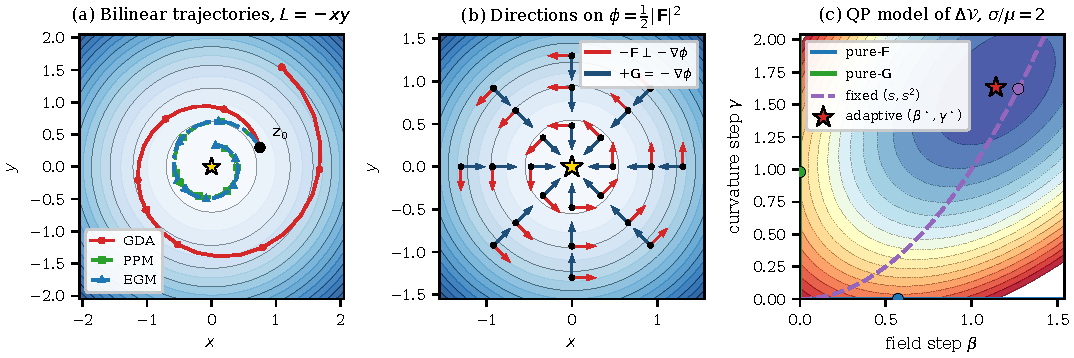
\includegraphics[width=0.94\textwidth]{output/pdf/fig_motivation_geometry.pdf}
		\caption{Analytical mechanism illustration from exact calculations.
			(a) On the bilinear game $L=-xy$, GDA
			spirals outward, whereas PPM and EGM contract toward the saddle
			($s=0.25$).
			(b) For $\bF(x,y)=(y,-x)$, $-\bF$ is tangent to the
			field-energy level sets, while
			$+\bG=\nabla\bF\,\bF=-\nabla\phi$ points inward.
			(c) The QP searches
			the nonnegative $(\beta,\gamma)$ plane rather than a coordinate ray or the
			fixed EGM coupling $(s,s^{2})$; contours use
			$\Vk=\phi$, $\mu=0.35$, $\sigma=0.70$, and $\bz=(1,-0.65)$ without
			step size caps.}
		\label{fig:motivation_geometry}
	\end{figure*}
	
	Fig.~\ref{fig:motivation_geometry} isolates the field geometry.
	Section~\ref{sec:experiments} tests the predicted skew threshold, the
	two-coordinate QP identity, and the performance consequences.
	
	\subsection{Adaptive stochastic recursion and equilibrium notion}\label{subsec:recursion_oracle_fixedpoint}
	
	Let $\hatF_k$ and $\hatG_k$ denote the stochastic field and curvature oracles
	at update $k$, respectively.
	We study the recursion
	\begin{equation}\label{eq:update}
		\bz_{k+1}
		=
		\bz_{k}-\beta_{k}\hatF_{k}+\gamma_{k}\hatG_{k},
	\end{equation}
	where $\beta_{k},\gamma_{k}\ge 0$ are adaptive step sizes selected by minimizing
	a local model of the one-step change in $\Vk$.
	Let $\mathscr{F}_{k}$ denote the filtration generated by all algorithmic history before the stochastic queries at iteration $k$.
	
	\begin{assumption}[Biased stochastic oracles]\label{ass:oracles}
		For every $k$,
		\[
		\hatF_{k}
		=
		\bF(\bz_{k})+\biasF_{k}+\noiseF_{k},
		\quad
		\hatG_{k}
		=
		\bG(\bz_{k})+\biasG_{k}+\noiseG_{k},
		\]
		where $\biasF_{k},\biasG_{k}$ are $\mathscr{F}_{k}$-measurable and $\E[\noiseF_{k}\mid\mathscr{F}_{k}]=\E[\noiseG_{k}\mid\mathscr{F}_{k}]=\bzero$.
		There exist finite $\mathscr{F}_{k}$-measurable scalars $\bar b^{F}_{k},\bar b^{G}_{k},\sigma_{2,k},\sigma_{3,k}\ge 0$ such that, almost surely,
		\begin{enumerate}[(a)]
			\item $\norm{\biasF_{k}}\le \bar b^{F}_{k}$ and $\norm{\biasG_{k}}\le \bar b^{G}_{k}$;
			\item $\E[\norm{\noiseF_{k}}^{2}+\norm{\noiseG_{k}}^{2}\mid\mathscr{F}_{k}]\le \sigma_{2,k}^{2}$;
			\item $\E[\norm{\hatF_{k}}^{3}+\norm{\hatG_{k}}^{3}\mid\mathscr{F}_{k}]\le \sigma_{3,k}^{3}$.
		\end{enumerate}
	\end{assumption}
	
	Assumption~\ref{ass:oracles} covers unbiased mini-batch estimators and biases from clipped surrogates, truncated rollouts, and finite-difference curvature oracles.
	Section~\ref{sec:impl} treats directional-secant and moment-smoothed estimates of this local model through the estimation-error bound in Proposition~\ref{prop:model_approx}.
	The convergence target is the population stationarity set $\mathcal Z^\star$.
	Section~\ref{sec:drift} defines the weighted stationarity residual used in the
	finite-time analysis.
	
	% ============================================================
	\section{Adaptive Step-Size Design from the One-Step Change in a Composite Lyapunov Function}\label{sec:drift}
	% ============================================================
	
	\subsection{Composite Lyapunov function and second-order expansion}\label{subsec:V_drift}
	Here, Lyapunov drift means the one-step change
	$\Vk(\bz_{k+1})-\Vk(\bz_k)$ in the function defined below.
	
	A small field norm need not imply a small policy-space gap.
	We therefore combine field energy with a regularized local saddle-gap term and
	an optional nonnegative task-specific error.
	
	\begin{definition}[Local proximal saddle-gap residual]\label{def:local_gap}
		Fix proximal parameters $\tau_{\theta},\tau_{\psi}>0$.
		For every $\bz$, let $\cB_{\theta}(\bz)$ and $\cB_{\psi}(\bz)$ be nonempty
		compact local neighborhoods containing $\btheta$ and $\bpsi$, respectively.
		For $\bz=(\btheta,\bpsi)$, define the maximizing and minimizing players' local proximal improvement gaps
		\begin{align*}
			\cG_{\theta,\tau}(\bz)
			&\triangleq
			\max_{\bar\btheta\in\cB_{\theta}(\bz)}
			\Bigl\{
			J(\bar\btheta,\bpsi)
			-\tfrac{1}{2\tau_{\theta}}\norm{\bar\btheta-\btheta}^{2}
			\Bigr\}
			-J(\btheta,\bpsi),\\
			\cG_{\psi,\tau}(\bz)
			&\triangleq
			J(\btheta,\bpsi)
			-\min_{\bar\bpsi\in\cB_{\psi}(\bz)}
			\Bigl\{
			J(\btheta,\bar\bpsi)
			+\tfrac{1}{2\tau_{\psi}}\norm{\bar\bpsi-\bpsi}^{2}
			\Bigr\},
		\end{align*}
		The compactness assumptions make the extrema well defined, and inclusion of the
		current parameters gives $\cG_{\theta,\tau}(\bz)\ge0$ and
		$\cG_{\psi,\tau}(\bz)\ge0$.
		Fix a smoothing parameter $\epsilon>0$.
		The regularized local saddle-gap residual is
		\[
		\cP_{\tau}(\bz)
		\triangleq
		\widetilde\sigma_{\epsilon}\!\bigl(\cG_{\theta,\tau}(\bz)\bigr)
		+
		\widetilde\sigma_{\epsilon}\!\bigl(\cG_{\psi,\tau}(\bz)\bigr),
		\]
		where
		\[
		\widetilde\sigma_{\epsilon}(u)
		\triangleq
		\epsilon\log\!\left(\frac{1+e^{u/\epsilon}}{2}\right),
		\quad u\ge0,
		\]
		is the centered softplus.
		It is $C^\infty$, nonnegative on the nonnegative gap domain,
		$\widetilde\sigma_{\epsilon}(0)=0$, and
		$0\le u-\widetilde\sigma_{\epsilon}(u)\le\epsilon\log2$ for $u\ge0$.
	\end{definition}
	
	Let $\cP$ denote the nonnegative $C^3$ performance component used by the
	controller.
	We take $\cP=\cP_\tau$ for the local realization above and
	$\cP=\operatorname{Gap}_{\varepsilon}$ when global regularized best responses
	are available.
	The latter bounds the maximizing player's worst-case-return suboptimality through
	\eqref{eq:performance_bridge}.
	
	\begin{remark}[Smooth realization of $\cP_{\tau}$]\label{rem:Ptau_smooth}
		The analysis requires the chosen function $\Vk$ to be $C^3$.
		For exact envelopes,
		this follows locally when the feasible-set parameterizations are $C^3$, the
		optimizers are unique and interior, and their second-order optimality matrices
		are nonsingular.
		A fixed differentiable inner loop also suffices when
		nonnegativity is enforced by construction.
		Hard safeguards require a fixed
		active set on the analyzed neighborhood.
	\end{remark}
	
	\begin{definition}[Composite Lyapunov function]\label{def:Lyap}
		Let $\eta_{\psi}>0$ and define the block-diagonal weight matrix
		\[
		\bW_{V}\triangleq\diag(\Id_{d_{\theta}},\,\eta_{\psi}\Id_{d_{\psi}})\in\R^{d\times d},
		\]
		where $\diag(\cdot)$ forms a block-diagonal matrix.
		The weighted field-energy component is $\cE_{F}(\bz)\triangleq\tfrac12\bF(\bz)^{\top}\bW_{V}\bF(\bz)$.
		Let $\cC(\bz)$ be any nonnegative $C^{3}$ task-specific scalar error.
		For fixed normalizers $\kappa_{F},\kappa_{P},\kappa_{C}>0$ and weights $\lambda_{F}>0$, $\lambda_{P}\ge0$, $\lambda_{C}\ge0$, define the composite Lyapunov function
		\begin{equation}\label{eq:Vdef}
			\Vk(\bz)
			\triangleq
			\lambda_{F}\frac{\cE_{F}(\bz)}{\kappa_{F}}
			+
			\lambda_{P}\frac{\cP(\bz)}{\kappa_{P}}
			+
			\lambda_{C}\frac{\cC(\bz)}{\kappa_{C}}.
		\end{equation}
		The experiments use a fixed numerical floor $\epsilon_0>0$ and initial-point
		normalizers, e.g., $\kappa_F=\cE_F(\bz_0)+\epsilon_0$,
		$\kappa_P=\cP(\bz_0)+\epsilon_0$, and
		$\kappa_C=\cC(\bz_0)+\epsilon_0$; they set $\lambda_C=0$.
	\end{definition}
	
	Here $\bW_{V}$ weights the two policy-gradient blocks and is unrelated to the antisymmetric Jacobian part
	$\bW=\skewop(\nabla\bF)$.
	All experiments use $\eta_\psi=1$, which gives $\cE_F=\phi$; a general
	$\eta_\psi$ permits fixed block scaling.
	Setting $\lambda_P=\lambda_C=0$ gives the field-energy-only special case used
	in Sections~\ref{subsec:controlled_geometry} and
	\ref{subsec:finite_trajectory}.
	The field-energy term is always present because $\lambda_F>0$.
	The other terms add performance or task-specific information.
	The conditions below ensure that the expected one-step change in $\Vk$ is negative
	up to stochastic and approximation errors.
	
	\begin{lemma}[Properties of the composite Lyapunov function]\label{lem:Lyap_properties}
		Suppose Assumption~\ref{ass:smooth} holds and $\cP,\cC$ are $C^{3}$ on $\cD$.
		Then:
		\begin{enumerate}[(a)]
			\item $\Vk(\bz)\ge 0$ on $\cD$, and since $\lambda_{F}>0$, $\Vk(\bz)=0$ implies $\bz\in\mathcal{Z}^{\star}$;
			\item $\Vk\in C^{3}(\cD)$;
			\item the gradient is
			$\nabla\Vk=(\lambda_F/\kappa_F)\nabla\cE_F
			+(\lambda_P/\kappa_P)\nabla\cP+(\lambda_C/\kappa_C)\nabla\cC$,
			where $\nabla\cE_F=\nabla\bF^{\top}\bW_V\bF$;
			\item $\Phi(\bz)\triangleq\bF(\bz)^{\top}\bW_{V}\bF(\bz)$ is the
			weighted stationarity residual and satisfies
			$\Phi(\bz)\le2\kappa_{F}\Vk(\bz)/\lambda_{F}$.
		\end{enumerate}
	\end{lemma}
	
	\begin{proof}
		See Appendix~\ref{app:proofs}.
	\end{proof}
	
	The implication $\Vk(\bz)=0\Rightarrow\bF(\bz)=0$ always holds.
	A positive gap term can keep $\Vk(\bz)>0$ at a stationary point.
	We use $\Vk$ to control the one-step update and $\Phi$ to measure first-order
	stationarity.
	
	For nonnegative $(\beta,\gamma)$, the trial displacement is $\Delta_{k}(\beta,\gamma)\triangleq -\beta\hatF_{k}+\gamma\hatG_{k}$.
	
	\begin{assumption}[Local regularity along the iterates]\label{ass:local_reg}
		For every $k$ and every feasible $(\beta,\gamma)$ produced by the step-size routine, the segment $\{\bz_{k}+t\Delta_{k}(\beta,\gamma):t\in[0,1]\}\subset\cD$.
		There exist $\mathscr{F}_{k}$-measurable
		$G_{V,k},H_{V,k},M_{3,k}\ge 0$ that, simultaneously for every feasible pair
		and almost every realization of the current stochastic queries, satisfy
		$\norm{\nabla\Vk(\bz_{k})}\le G_{V,k}$,
		$\norm{\nabla^{2}\Vk(\bz_{k})}\le H_{V,k}$, and
		$\sup_{t\in[0,1]}\norm{\nabla^{3}\Vk(\bz_{k}+t\Delta_{k}(\beta,\gamma))}
		\le M_{3,k}$.
	\end{assumption}
	
	The five local-model terms are
	\begin{equation}\label{eq:drift_terms_def}
		\begin{aligned}
			e_{k}&\triangleq\inner{\nabla\Vk(\bz_{k})}{\hatF_{k}},
			\quad
			d_{k}\triangleq -\inner{\nabla\Vk(\bz_{k})}{\hatG_{k}},\\
			c_{k}&\triangleq\hatF_{k}^{\top}\nabla^{2}\Vk(\bz_{k})\hatF_{k},
			\quad
			a_{k}\triangleq\hatG_{k}^{\top}\nabla^{2}\Vk(\bz_{k})\hatG_{k},\\
			b_{k}&\triangleq\hatF_{k}^{\top}\nabla^{2}\Vk(\bz_{k})\hatG_{k}.
		\end{aligned}
	\end{equation}
	These terms are directional derivatives of $\Vk$ in~\eqref{eq:Vdef}.
	Thus, the quadratic model accounts for every selected component of $\Vk$
	rather than only field energy.
	
	\begin{lemma}[Second-order expansion of the one-step change in $\Vk$]\label{lem:drift_taylor}
		Under Assumption~\ref{ass:local_reg}, for every feasible $(\beta,\gamma)$,
		\begin{equation}\label{eq:drift_taylor}
			\begin{aligned}
				&\Vk(\bz_{k}+\Delta_{k}(\beta,\gamma))-\Vk(\bz_{k}) \\
				&=
				-\beta e_{k}-\gamma d_{k}
				+\tfrac{1}{2}c_{k}\beta^{2}-b_{k}\beta\gamma+\tfrac{1}{2}a_{k}\gamma^{2}
				+\mathrm{rem}_{k}(\beta,\gamma),
			\end{aligned}
		\end{equation}
		with $\lvert \mathrm{rem}_{k}(\beta,\gamma)\rvert\le\frac{M_{3,k}}{6}(\beta\norm{\hatF_{k}}+\gamma\norm{\hatG_{k}})^{3}$.
	\end{lemma}
	
	\begin{proof}
		See Appendix~\ref{app:proofs}.
	\end{proof}
	
	The five local terms in this lemma define the QP below.
	
	\subsection{Implemented quadratic subproblem and closed-form solution}\label{subsec:closed_form}
	Let $(\hat e_k,\hat d_k,\hat c_k,\hat a_k,\hat b_k)$ denote the stabilized
	local-model terms constructed below.
	With nonnegative diagonal stabilizers $\rho_{a,k},\rho_{c,k}\ge 0$, the implemented quadratic model of the change in $\Vk$ is
	\begin{equation}\label{eq:qhat}
		\begin{aligned}
			\hat q_{k}(\beta,\gamma)
			&\triangleq
			-\beta\hat e_{k}-\gamma\hat d_{k}
			+\tfrac{1}{2}\hat c_{k}\beta^{2}-\hat b_{k}\beta\gamma\\
			&\quad+\tfrac{1}{2}\hat a_{k}\gamma^{2},
			\quad (\beta,\gamma)\in\R_{+}^{2},
		\end{aligned}
	\end{equation}
	where Section~\ref{sec:impl} supplies raw estimates
	$(\tilde e_k,\tilde d_k,\tilde c_k,\tilde a_k,\tilde b_k)$ of
	$(e_k,d_k,c_k,a_k,b_k)$.
	For a scalar $u$, let $[u]_+\triangleq\max\{u,0\}$.
	For a fixed $\lambda_{\rm pd}>0$, define
	\[
		\widetilde{\bH}_k
		=
		\begin{bmatrix}
			\tilde c_k&-\tilde b_k\\
			-\tilde b_k&\tilde a_k
		\end{bmatrix}.
	\]
	We set
	\[
		\lambda_k=[\lambda_{\rm pd}-\lambda_{\min}(\widetilde{\bH}_k)]_+,
		\qquad
		\widehat{\bH}_k=\widetilde{\bH}_k+\lambda_k\Id_2.
	\]
	We then set $\hat e_k=\tilde e_k$, $\hat d_k=\tilde d_k$,
	$\hat b_k=\tilde b_k$, $\hat c_k=\tilde c_k+\lambda_k$,
	$\hat a_k=\tilde a_k+\lambda_k$, and
	$\rho_{c,k}=\rho_{a,k}=\lambda_k$.
	Then $\hat\delta_k\triangleq\det\widehat{\bH}_k
	=\hat c_k\hat a_k-\hat b_k^2$, and
	$(\beta_k^\star,\gamma_k^\star)$ minimizes $\hat q_k$ over $\R_+^2$.
	
	\begin{assumption}[Positive definiteness]\label{ass:PD}
		For every $k$, $\widehat{\bH}_{k}\succ 0$, equivalently $\hat c_{k}>0$ and $\hat\delta_{k}>0$.
	\end{assumption}
	
	The common spectral shift above gives
	$\widehat{\bH}_k\succeq\lambda_{\rm pd}\Id_2$ and therefore enforces
	Assumption~\ref{ass:PD}.
	The unconstrained critical point is
	\begin{equation}\label{eq:unconstrained_pair}
		(\beta_{k}^{\rm uc},\gamma_{k}^{\rm uc})
		\triangleq
		\Bigl(\tfrac{\hat a_{k}\hat e_{k}+\hat b_{k}\hat d_{k}}{\hat\delta_{k}},\,
		\tfrac{\hat b_{k}\hat e_{k}+\hat c_{k}\hat d_{k}}{\hat\delta_{k}}\Bigr),
	\end{equation}
	and the boundary candidates are $\bigl([\hat e_{k}/\hat c_{k}]_{+},0\bigr)$, $\bigl(0,[\hat d_{k}/\hat a_{k}]_{+}\bigr)$, $(0,0)$.
	
	\begin{theorem}[Closed-form implemented step-size rule]\label{thm:closed_form}
		Under Assumption~\ref{ass:PD}, the implemented problem~\eqref{eq:qhat} admits a unique minimizer, given by~\eqref{eq:unconstrained_pair} when both components are nonnegative, and otherwise by the boundary candidate with smallest $\hat q_{k}$.
		When the unconstrained critical point belongs to $\R_+^2$, the implemented predicted decrease $\widehat\Delta_{k}^{\star}\triangleq -\hat q_{k}(\beta_{k}^{\star},\gamma_{k}^{\star})$ is
		\begin{equation}\label{eq:Delta_hat_interior}
			\widehat\Delta_{k}^{\star}=\frac{\hat a_{k}\hat e_{k}^{2}+2\hat b_{k}\hat e_{k}\hat d_{k}+\hat c_{k}\hat d_{k}^{2}}{2\hat\delta_{k}}.
		\end{equation}
	\end{theorem}
	
	\begin{proof}
		See Appendix~\ref{app:proofs}.
	\end{proof}
	
	Because the subproblem is two-dimensional, the unconstrained formula and
	boundary fallback use a fixed number of scalar operations.
	The rule depends only on the current local model estimates.
	
	\begin{proposition}[Exact box-constrained fallback]\label{prop:box_fallback}
		Under Assumption~\ref{ass:PD}, fix finite caps $\beta_{\max},\gamma_{\max}>0$.
		The unique minimizer of $\hat q_k$ on
		$[0,\beta_{\max}]\times[0,\gamma_{\max}]$ is the member with smallest objective
		value among the feasible unconstrained point~\eqref{eq:unconstrained_pair} and the four
		edge minimizers
		\begin{align*}
			&\left(\left[\hat e_k/\hat c_k\right]_{[0,\beta_{\max}]},0\right),\quad
			\left(0,\left[\hat d_k/\hat a_k\right]_{[0,\gamma_{\max}]}\right),\\
			&\left(\beta_{\max},
			\left[(\hat d_k+\hat b_k\beta_{\max})/\hat a_k\right]_{[0,\gamma_{\max}]}\right),\\
			&\left(\left[(\hat e_k+\hat b_k\gamma_{\max})/\hat c_k\right]_{[0,\beta_{\max}]},
			\gamma_{\max}\right),
		\end{align*}
		where $[u]_{[l,r]}\triangleq\min\{r,\max\{l,u\}\}$.
		Consequently its predicted decrease dominates every one-direction or
		fixed-coupling comparator whose step size pair lies in the same box.
	\end{proposition}
	\begin{proof}
		Strict convexity gives a unique minimizer.
		If it is in the interior, the gradient equations give~\eqref{eq:unconstrained_pair};
		otherwise it lies on one of the four edges, and differentiating the resulting
		one-dimensional strictly convex quadratic and clipping its stationary point
		to that edge gives the four displayed candidates.
		Set inclusion then proves the dominance statement.
	\end{proof}
	
	\subsection{Predicted-decrease dominance and its geometric meaning}\label{subsec:dominance}
	
	\begin{theorem}[Predicted-decrease dominance]\label{thm:dominance}
		Under Assumption~\ref{ass:PD}, fix $s_{\max}>0$ and define
		\begin{align*}
			\widehat\Delta_{k}^{\bF}
			&\triangleq
			-\min_{\beta\ge 0}\hat q_{k}(\beta,0)
			=
			\tfrac{[\hat e_{k}]_{+}^{2}}{2\hat c_{k}},\\
			\widehat\Delta_{k}^{\bG}
			&\triangleq
			-\min_{\gamma\ge 0}\hat q_{k}(0,\gamma)
			=
			\tfrac{[\hat d_{k}]_{+}^{2}}{2\hat a_{k}},\\
			\widehat\Delta_{k}^{\mathrm{2nd}}
			&\triangleq
			-\min_{s\in[0,s_{\max}]}\hat q_{k}(s,s^{2}),
		\end{align*}
		Then $\widehat\Delta_{k}^{\star}\ge\max\{\widehat\Delta_{k}^{\bF},\widehat\Delta_{k}^{\bG},\widehat\Delta_{k}^{\mathrm{2nd}}\}$ almost surely.
		Moreover, when the unconstrained critical point~\eqref{eq:unconstrained_pair}
		belongs to $\R_+^2$, the gap over the pure-field rule is exactly
		\begin{equation}\label{eq:dominance_gap}
			\widehat\Delta_{k}^{\star}-\widehat\Delta_{k}^{\bF}
			=
			\frac{(\hat b_{k}\hat e_{k}+\hat c_{k}\hat d_{k})^{2}}{2\hat c_{k}\hat\delta_{k}}
			+\frac{[-\hat e_k]_{+}^{2}}{2\hat c_k}
			\ge 0,
		\end{equation}
		which is strictly positive if and only if either $\hat b_{k}\hat e_{k}+\hat c_{k}\hat d_{k}\neq 0$ or $\hat e_k<0$.
		In the usual field-descent regime $\hat e_k\ge0$, strict improvement is therefore equivalent to the curvature direction having a nonzero reduced gradient after projecting out the field direction in the $\widehat{\bH}_{k}$-metric.
	\end{theorem}
	
	\begin{proof}
		See Appendix~\ref{app:proofs}.
	\end{proof}
	
	At an interior solution, \eqref{eq:dominance_gap} quantifies the extra predicted
	decrease supplied by the curvature coordinate.
	The reduced gradient $\hat b_{k}\hat e_{k}+\hat c_{k}\hat d_{k}$ is the
	component that remains after accounting for the field direction in the local
	quadratic model.
	If $\bG$ is collinear with $\bF$, the two directions span one geometric
	direction.
	With zero diagonal inflation, the associated two-coordinate Hessian is
	singular.
	Any QP gain in this case comes from step size constraints or regularization,
	not span enlargement.
	In the field-descent regime $\hat e_k\ge0$, antisymmetry alone is insufficient:
	strict interior improvement also requires a nonzero reduced descent component.
	Assumption~\ref{ass:margin} measures this improvement in the stochastic
	stationarity bound.
	
	\subsection{Pathwise one-step bound and per-iteration error}\label{subsec:pathwise}
	The implemented model is allowed to differ from the reference quadratic
	\[
	\begin{aligned}
		q_{k}(\beta,\gamma)
		\triangleq{}&-\beta e_{k}-\gamma d_{k}
		+\tfrac{1}{2}(c_{k}+\rho_{c,k})\beta^{2}\\
		&-b_{k}\beta\gamma
		+\tfrac{1}{2}(a_{k}+\rho_{a,k})\gamma^{2}
	\end{aligned}
	\]
	through a one-sided model-consistency residual.
	Define the cubic Taylor remainder
	$\varepsilon_{k}^{\mathrm{rem}}\triangleq M_{3,k}
	(\beta_{k}\norm{\hatF_{k}}+\gamma_{k}\norm{\hatG_{k}})^{3}/6$.
	Let $\varepsilon_k^{\rm model}\ge0$ be $\mathscr F_{k+1}$-measurable and satisfy
	$q_k(\beta_k,\gamma_k)\le\hat q_k(\beta_k,\gamma_k)
	+\varepsilon_k^{\rm model}$, and set
	$\varepsilon_k^{\rm step}\triangleq\hat q_k(\beta_k,\gamma_k)
	+\widehat\Delta_k^\star\ge0$.
	The total per-iteration residual is
	\begin{equation}\label{eq:eps_tot}
		\varepsilon_{k}^{\mathrm{tot}}\triangleq\varepsilon_{k}^{\mathrm{rem}}+\varepsilon_{k}^{\mathrm{model}}+\varepsilon_{k}^{\mathrm{step}},
	\end{equation}
	The residual $\varepsilon_{k}^{\mathrm{model}}$ vanishes for exact autodifferentiation and admits an explicit bound for approximate realizations through Proposition~\ref{prop:model_approx}; $\varepsilon_{k}^{\mathrm{step}}$ vanishes for the unsafeguarded closed-form rule.
	
	\begin{lemma}[Pathwise bound on the one-step change in $\Vk$]\label{lem:pathwise_drift}
		Under Assumptions~\ref{ass:local_reg} and~\ref{ass:PD}, for every $k$,
		\begin{equation}\label{eq:pathwise_drift}
			\Vk(\bz_{k+1})-\Vk(\bz_{k})\le -\widehat\Delta_{k}^{\star}+\varepsilon_{k}^{\mathrm{tot}}\quad\text{almost surely}.
		\end{equation}
	\end{lemma}
	
	\begin{proof}
		See Appendix~\ref{app:proofs}.
	\end{proof}
	
	The inequality separates model decrease from implementation residuals.
	
	\begin{lemma}[Conditional residual bound]\label{lem:residual_budget}
		Suppose Assumptions~\ref{ass:oracles} and~\ref{ass:local_reg} hold and $\beta_{k}\le\beta_{\max}$, $\gamma_{k}\le\gamma_{\max}$.
		Then
		\begin{equation}\label{eq:eps_rem_cond}
			\E[\varepsilon_{k}^{\mathrm{rem}}\mid\mathscr{F}_{k}]
			\le
			\frac{2M_{3,k}}{3}(\beta_{\max}+\gamma_{\max})^{3}\sigma_{3,k}^{3}.
		\end{equation}
		If additionally $M_{3,k}\le\bar M_{3}$ and $\sigma_{3,k}\le\bar\sigma_{3}$, then $\E[\varepsilon_{k}^{\mathrm{rem}}]$ is uniformly bounded.
	\end{lemma}
	
	\begin{proof}
		See Appendix~\ref{app:proofs}.
	\end{proof}
	
	Thus the cubic remainder has a finite conditional expectation under the stated
	moment bound.
	
	% ============================================================
	\section{Expected One-Step Change and Convergence Analysis}\label{sec:conv}
	% ============================================================
	
	\subsection{Local admissible region and structural conditions}\label{subsec:local_assumps}
	Recall the weighted stationarity residual
	\[
	\begin{aligned}
		\Phi(\bz)
		&\triangleq
		\bF(\bz)^{\top}\bW_{V}\bF(\bz)\\
		&=
		\norm{\nabla_{\btheta}J}^{2}
		+\eta_{\psi}\norm{\nabla_{\bpsi}J}^{2},
	\end{aligned}
	\]
	which vanishes precisely on $\mathcal{Z}^{\star}$.
	
	\begin{assumption}[Local admissible region and Lyapunov decrease]\label{ass:local}
		There exist an open admissible set $\cN$ whose compact closure satisfies
		$\overline{\cN}\subset\cD$, an index $k_{0}\ge 0$, and constants
		$\mu_{\Phi}\ge0$, $\mu_{V}\ge0$ such that $\cN$ contains the local trajectory
		after $k_{0}$ together with the stationary component of $\mathcal{Z}^{\star}$
		under consideration, and:
		\begin{enumerate}[(a)]
			\item $\bz_{k}\in\cN$ for all $k\ge k_{0}$ almost surely;
			\item $\inner{\nabla\Vk(\bz)}{\bF(\bz)}\ge \mu_{\Phi}\Phi(\bz)$ for all $\bz\in\cN$;
			\item when geometric contraction is invoked, $\inner{\nabla\Vk(\bz)}{\bF(\bz)}\ge \mu_{V}\Vk(\bz)$ for all $\bz\in\cN$.
		\end{enumerate}
	\end{assumption}
	
	Because the algorithm moves along $-\bF$, condition (b) states that this
	direction decreases $\Vk$ at least in proportion to the stationarity residual
	$\Phi$.
	Combined with the conditional bound below on the expected one-step change in
	$\Vk$, it gives the finite-time stationarity result.
	It plays the role of a Polyak--\L{}ojasiewicz (PL) inequality in a gradient system
	\cite{Karimi2016PL}.
	Condition (a) is a local invariance assumption.
	A prescribed trust region and backtracking can keep trial points in a chosen
	compact region.
	The analysis requires that region to satisfy (b)--(c).
	Condition (c) strengthens the required decrease from a multiple of $\Phi$ to a
	multiple of $\Vk$ itself; this stronger condition gives geometric contraction of
	$\E[\Vk]$.
	It requires $\Vk$ to vanish on the target component, excluding stationary points
	with a positive local gap from the contraction result.
	
	\begin{lemma}[Sufficient condition for Lyapunov decrease]\label{lem:local_PL_sufficient}
		Suppose Assumption~\ref{ass:smooth} holds and there exist $m_{F}>0$ and $\delta_{P},\delta_{C}\ge0$ such that, for all $\bz\in\cN$,
		\begin{equation}\label{eq:sym_part_pd}
			\bF(\bz)^{\top}\sym\!\bigl(\bW_{V}\nabla\bF(\bz)\bigr)\bF(\bz)
			\ge
			m_{F}\,\bF(\bz)^{\top}\bW_{V}\bF(\bz),
		\end{equation}
		and
		\begin{equation}\label{eq:gap_aux_negative_bound}
			\begin{aligned}
				\frac{\lambda_{P}}{\kappa_{P}}\inner{\nabla\cP(\bz)}{\bF(\bz)}
				&+
				\frac{\lambda_{C}}{\kappa_{C}}\inner{\nabla\cC(\bz)}{\bF(\bz)}
				\\
				&\ge
				-(\delta_{P}+\delta_{C})\Phi(\bz).
			\end{aligned}
		\end{equation}
		If $\lambda_{F}m_{F}/\kappa_{F}>\delta_{P}+\delta_{C}$, then
		Assumption~\ref{ass:local}(b) holds with
		\[
		\mu_{\Phi}
		=\lambda_{F}m_{F}/\kappa_{F}-\delta_{P}-\delta_{C}>0.
		\]
	\end{lemma}
	
	\begin{proof}
		See Appendix~\ref{app:proofs}.
	\end{proof}
	
	\begin{remark}[Compatibility of the Lyapunov components]\label{rem:weight_constraint}
		Eq.~\eqref{eq:sym_part_pd} is positivity of the weighted symmetric
		Jacobian along $\bF$; in the canonical unweighted pure-rotation case
		$\bW_V=\Id$, one has $m_F=0$.
		Bounded gap gradients alone
		do not imply~\eqref{eq:gap_aux_negative_bound}, whose right side is
		$O(\norm{\bF}^2)$: the negative gap/auxiliary derivatives must vanish at least
		linearly with $\bF$.
		The resulting $\delta_P,\delta_C$ scale with their
		component weights, making the displayed strict inequality an explicit
		compatibility condition.
	\end{remark}
	
	Because $\overline{\cN}$ is compactly contained in $\cD$, continuity of the
	relevant derivatives yields uniform constants $G_{V},H_{V},B_{F}\ge 0$ with
	$\norm{\nabla\Vk(\bz)}\le G_{V}$,
	$\norm{\nabla^{2}\Vk(\bz)}\le H_{V}$, and
	$\norm{\bF(\bz)}\le B_{F}$ for all $\bz\in\cN$; in particular
	$G_{V,k},H_{V,k}$ may be replaced by $G_{V},H_{V}$ for $k\ge k_{0}$.
	
	\begin{assumption}[Uniform residual budget on $\cN$]\label{ass:budget}
		There exist finite $\bar b_{F},\bar b_{G},\bar\sigma_{2},\bar\rho_{c},\bar R\ge0$
		such that, for all $k\ge k_{0}$:
		\begin{enumerate}[(a)]
			\item $\bar b^{F}_{k}\le\bar b_{F}$,
			$\bar b^{G}_{k}\le\bar b_{G}$, and $\sigma_{2,k}\le\bar\sigma_{2}$;
			\item $\rho_{c,k}\le\bar\rho_{c}$;
			\item $\E[\varepsilon_{k}^{\mathrm{tot}}]\le \bar R$.
		\end{enumerate}
	\end{assumption}
	
	The baseline one-step and stationarity results first use exact local-model terms,
	$\hat e_k=\inner{\nabla\Vk(\bz_k)}{\hatF_k}$ and
	$\hat c_k=\hatF_k^\top\nabla^2\Vk(\bz_k)\hatF_k+\rho_{c,k}$.
	The curvature-improvement theorem then retains box constraints, local-model estimation error,
	and safeguard loss explicitly.
	
	\subsection{Expected one-step change under biased oracles}\label{subsec:cond_drift}
	Define the second-moment field bound $M_{F}\triangleq 3B_{F}^{2}+3\bar b_{F}^{2}+3\bar\sigma_{2}^{2}$.
	
	\begin{theorem}[Expected one-step change in $\Vk$]\label{thm:cond_drift}
		Suppose Assumptions~\ref{ass:smooth}, \ref{ass:oracles}, \ref{ass:local_reg}, \ref{ass:PD}, and~\ref{ass:budget} hold, the algorithm uses the exact-autodifferentiation realization, and the iterates satisfy $\bz_{k}\in\cN$ for all $k\ge k_{0}$ as in Assumption~\ref{ass:local}(a). The uniform bounds $G_{V},H_{V},M_{F}$ are then valid on $\cN$.
		Then for every $k\ge k_{0}$ and every deterministic $\bar\beta\ge 0$,
		\begin{equation}\label{eq:cond_drift}
			\begin{aligned}
				&\E[\Vk(\bz_{k+1})-\Vk(\bz_{k})\mid\mathscr{F}_{k}]\\
				&\le
				-\bar\beta\inner{\nabla\Vk(\bz_{k})}{\bF(\bz_{k})}+\bar\beta G_{V}\bar b_{F} \\
				&+\tfrac{1}{2}\bar\beta^{2}
				\bigl(H_{V}M_{F}+\bar\rho_{c}\bigr)\\
				&+\E[\varepsilon_{k}^{\mathrm{tot}}\mid\mathscr{F}_{k}].
			\end{aligned}
		\end{equation}
	\end{theorem}
	
	\begin{proof}
		See Appendix~\ref{app:proofs}.
	\end{proof}
	
	The reference scalar $\bar\beta\ge 0$ is an analytical comparator.
	The proof removes the curvature-oracle bias $\bar b_G$ from
	\eqref{eq:cond_drift} by restricting the predicted decrease to the
	pure-$\bF$ coordinate, which uses $\hat e_k$ and $\hat c_k$.
	Define the error term $\mathcal{R}(\bar\beta)\triangleq \bar\beta G_{V}\bar b_{F}+\tfrac{1}{2}\bar\beta^{2}(H_{V}M_{F}+\bar\rho_{c})+\bar R$.
	
	\subsection{Finite-time average stationarity and contraction}\label{subsec:ergodic}
	
	\begin{theorem}[Local finite-time average stationarity]\label{thm:ergodic}
		Under the assumptions of Theorem~\ref{thm:cond_drift}, suppose additionally that Assumption~\ref{ass:local}(b) holds with $\mu_\Phi>0$.
		Then, for every $\bar\beta>0$ and integer $K>k_{0}$,
		\begin{equation}\label{eq:main_stationarity}
			\frac{1}{K-k_{0}}
			\sum_{k=k_{0}}^{K-1}\E[\Phi(\bz_{k})]
			\le
			\frac{\E[\Vk(\bz_{k_{0}})]}{\bar\beta\mu_{\Phi}(K-k_{0})}
			+
			\frac{\mathcal{R}(\bar\beta)}{\bar\beta\mu_{\Phi}}.
		\end{equation}
	\end{theorem}
	
	\begin{proof}
		See Appendix~\ref{app:proofs}.
	\end{proof}
	
	The left side of Eq.~\eqref{eq:main_stationarity} is the Ces\`aro, or time,
	average of the expected stationarity residuals.
	If $I_K$ is uniform on $\{k_0,\ldots,K-1\}$ and independent of the algorithm,
	this average equals $\E[\Phi(\bz_{I_K})]$.
	Thus the expected residual of a uniformly selected iterate has an
	$O(1/(K-k_0))$ transient plus the stated error floor; the policy parameters are
	not averaged.
	
	Theorems~\ref{thm:cond_drift}--\ref{thm:ergodic} use only
	$\widehat\Delta_k^\star\ge\widehat\Delta_k^{\bF}$.
	Assumption~\ref{ass:margin} lower-bounds the extra decrease in the local model of
	$\Vk$ from the curvature step size by the stationarity residual.
	It applies directly to the implemented box-QP, including active caps.
	For fixed caps $\beta_{\max},\gamma_{\max}>0$, define
	\begin{align*}
		\widehat\Delta_k^{\rm box}
		&\triangleq
		-\min_{\substack{0\le\beta\le\beta_{\max}\\
				0\le\gamma\le\gamma_{\max}}}\hat q_k(\beta,\gamma),\\
		\widehat\Delta_k^{F,\rm box}
		&\triangleq
		-\min_{0\le\beta\le\beta_{\max}}\hat q_k(\beta,0).
	\end{align*}
	
	\begin{assumption}[Expected model improvement from the curvature direction]\label{ass:margin}
		There exist $C_G>0$, $\bar r_G<\infty$, and nonnegative
		$\mathscr F_k$-measurable variables $r_{G,k}^{\rm mar}$ such that, for every
		$k\ge k_0$ almost surely,
		\begin{equation}\label{eq:margin}
			\E[\mathfrak D_{G,k}^{\rm box}\mid\mathscr F_k]
			\ge C_G\Phi(\bz_k)-r_{G,k}^{\rm mar},
			\quad
			\E[r_{G,k}^{\rm mar}]\le\bar r_G,
		\end{equation}
		where $\mathfrak D_{G,k}^{\rm box}\triangleq
		\widehat\Delta_k^{\rm box}-\widehat\Delta_k^{F,\rm box}$.
	\end{assumption}
	
	The quantity $\mathfrak D_{G,k}^{\rm box}$ is the extra decrease in the local
	model of $\Vk$ obtained when the QP optimizes both step sizes instead of fixing
	$\gamma=0$.
	The solved subproblem gives this quantity directly.
	Eq.~\eqref{eq:margin} requires its conditional mean to grow at least as fast as
	the population stationarity residual $\Phi$, up to $r_{G,k}^{\rm mar}$.
	A pathwise cap-valid certificate, which implies
	Assumption~\ref{ass:margin} with $r_{G,k}^{\rm mar}=0$, follows by letting
	$\hat\beta_k^F$ be the pure-field box minimizer and setting
	$r_{G,k}^{\rm box}=\hat d_k+\hat b_k\hat\beta_k^F$.
	The feasible comparator
	$(\hat\beta_k^F,\tilde\gamma)$ gives, for
	$0\le\tilde\gamma\le\gamma_{\max}$,
	\[
	\mathfrak D_{G,k}^{\rm box}\ge
	\tilde\gamma r_{G,k}^{\rm box}-\tfrac12\hat a_k\tilde\gamma^2.
	\]
	Thus, if on $\cN$, $0\le\Phi\le\bar\Phi>0$,
	$0<\hat a_k\le\bar a$, and
	$r_{G,k}^{\rm box}\ge m_G\sqrt{\Phi(\bz_k)}$, choosing
	$\tilde\gamma=\min\{\gamma_{\max},r_{G,k}^{\rm box}/\hat a_k\}$
	proves~\eqref{eq:margin} with
	\[
	C_G=\min\!\left\{\frac{m_G^2}{2\bar a},
	\frac{\gamma_{\max}m_G}{2\sqrt{\bar\Phi}}\right\}.
	\]
	Indeed, the comparator decrease is respectively
	$(r_{G,k}^{\rm box})^2/(2\hat a_k)$ before saturation and at least
	$\gamma_{\max}r_{G,k}^{\rm box}/2$ after it.
	For the uncapped problem, the sharper reduced coordinates
	$r_{G,k}=\hat d_k+\hat b_k\hat e_k/\hat c_k$ and
	$h_{G,k}=\hat a_k-\hat b_k^2/\hat c_k$ give
	$\mathfrak D_{G,k}=r_{G,k}^2/(2h_{G,k})
	+[-\hat e_k]_+^2/(2\hat c_k)\ge r_{G,k}^2/(2h_{G,k})$ whenever the
	unconstrained critical point is nonnegative.
	Hence
	$|r_{G,k}|\ge m_G\sqrt{\Phi}$ and
	$0<h_{G,k}\le\bar h_G$ give $C_G=m_G^2/(2\bar h_G)$.
	For the exact field-energy function and exact local-model terms, with no additional
	inflation, $\Vk=\phi=\tfrac12\|\bF\|^2$, $\bW_V=\Id$, and the pure rotation
	$\bF(\bz)=\sigma J_{0}(\bz-\bz^\star)$, a cap gives
	$C_G=\bar\gamma\sigma^{2}-\bar\gamma^{2}\sigma^{4}/2$ with
	$\bar\gamma=\min\{\gamma_{\max},\sigma^{-2}\}$.
	This expression reduces to $\bar\gamma-\bar\gamma^{2}/2$ when $\sigma=1$.
	
	\begin{theorem}[Stochastic stationarity bound with curvature improvement]\label{thm:curv_improved}
		Suppose Assumptions~\ref{ass:smooth}, \ref{ass:oracles},
		\ref{ass:local_reg}, \ref{ass:PD}, \ref{ass:local}(a)--(b), and
		\ref{ass:margin} hold, with $\mu_\Phi\ge0$, and the uniform bounds in
		Assumption~\ref{ass:budget}(a)--(b) hold.
		Suppose the accepted boxed pair satisfies
		$\hat q_k(\beta_k,\gamma_k)\le-\widehat\Delta_k^{\rm box}
		+\varepsilon_k^{\rm step,box}$ and
		\[
		\E[\varepsilon_k^{\rm rem}+\varepsilon_k^{\rm model}
		+\varepsilon_k^{\rm step,box}]\le\bar R_{\rm box}.
		\]
		If the estimation errors of Proposition~\ref{prop:model_approx} satisfy
		$\E[\delta_{e,k}\mid\mathscr F_k]\le\bar\delta_e$ and
		$\E[\delta_{c,k}\mid\mathscr F_k]\le\bar\delta_c$, define
		\[
		\begin{aligned}
			\mathcal R_{\rm box}(\bar\beta)
			={}&\bar\beta(G_V\bar b_F+\bar\delta_e)
			+\bar\beta^2(H_VM_F+\bar\rho_c+\bar\delta_c)/2\\
			&+\bar R_{\rm box}+\bar r_G.
		\end{aligned}
		\]
		Then, for every deterministic $\bar\beta\in[0,\beta_{\max}]$ with
		$\bar\beta\mu_\Phi+C_G>0$ and every integer $K>k_0$,
		\begin{equation}\label{eq:curv_improved}
			\begin{aligned}
				\frac{1}{K-k_{0}}\sum_{k=k_{0}}^{K-1}\E[\Phi(\bz_{k})]
				\le{}&
				\frac{\E[\Vk(\bz_{k_{0}})]}{(\bar\beta\mu_{\Phi}+C_G)(K-k_{0})}
				\\
				&+
				\frac{\mathcal{R}_{\rm box}(\bar\beta)}
				{\bar\beta\mu_{\Phi}+C_G}.
			\end{aligned}
		\end{equation}
	\end{theorem}
	
	\begin{proof}
		See Appendix~\ref{app:proofs}.
	\end{proof}
	
	The constant $C_G$ increases the weight multiplying $\Phi$ in the
	stationarity bound from $\bar\beta\mu_\Phi$ to
	$\bar\beta\mu_\Phi+C_G$.
	The resulting error floor is
	$\mathcal R_{\rm box}(\bar\beta)/(\bar\beta\mu_\Phi+C_G)$.
	
	\begin{corollary}[Local geometric contraction]\label{cor:local}
		In addition to the assumptions of Theorem~\ref{thm:cond_drift}, suppose Assumption~\ref{ass:local}(c) holds with $\mu_{V}>0$.
		Then for every $\bar\beta\in(0,1/\mu_{V}]$ and every $k\ge k_{0}$,
		\[
		\E[\Vk(\bz_{k})]
		\le
		(1-\bar\beta\mu_{V})^{k-k_{0}}\E[\Vk(\bz_{k_{0}})]
		+
		\frac{\mathcal{R}(\bar\beta)}{\bar\beta\mu_{V}}.
		\]
	\end{corollary}
	
	\begin{proof}
		See Appendix~\ref{app:proofs}.
	\end{proof}
	
	\begin{corollary}[Worst-case return and Nash-gap bound]\label{cor:performance_contraction}
		Suppose the assumptions of Corollary~\ref{cor:local} hold, $\mathcal A$ and
		$\mathcal B$ are finite, $\lambda_P>0$, and
		$\cP=\operatorname{Gap}_\varepsilon$ in Eq.~\eqref{eq:Vdef}.
		For $\bar\beta\in(0,1/\mu_V]$, write
		$q_{\bar\beta}=1-\bar\beta\mu_V$ and
		$B_\varepsilon=\varepsilon(\log|\mathcal A|+\log|\mathcal B|)/(1-\alpha)$.
		Then, for every $k\ge k_0$,
		\begin{equation}\label{eq:performance_contraction}
			\begin{aligned}
				\E[v^\star-R_{\rm BR}(\pi_{\btheta_k})]
				&\le \E[\operatorname{Gap}_0(\bz_k)]\\
				&\le \frac{\kappa_P}{\lambda_P}\left[
				q_{\bar\beta}^{k-k_0}\E[\Vk(\bz_{k_0})]
				+\frac{\mathcal R(\bar\beta)}{\bar\beta\mu_V}\right]
				+B_\varepsilon.
			\end{aligned}
		\end{equation}
	\end{corollary}
	
	\begin{proof}
		Eq.~\eqref{eq:Vdef} gives
		$\operatorname{Gap}_\varepsilon(\bz_k)\le
		(\kappa_P/\lambda_P)\Vk(\bz_k)$.
		Apply Corollary~\ref{cor:local} and then
		Proposition~\ref{prop:performance_bridge}.
	\end{proof}
	
	% ============================================================
	\section{Local-Model Realizations and Implementation}\label{sec:impl}
	% ============================================================
	
	\subsection{Exact local-model evaluation}
	The terms in~\eqref{eq:drift_terms_def} are assembled from one field oracle $\hatF_{k}$, one curvature oracle $\hatG_{k}$, one gradient $\nabla\Vk(\bz_k)$, and the Hessian--vector products of $\Vk$ along $\hatF_k$ and $\hatG_k$.
	When a fixed differentiable inner loop implements $\cP$, autodifferentiation
	passes through it; implicit differentiation handles an exact local envelope.
	Because the field-energy component contains $\bF^\top\bW_V\bF/2$, exact
	Hessian--vector products of $\Vk$ generally involve third derivatives of the
	underlying game objective; the secant realization below avoids constructing
	those derivatives.
	For exact local-model terms, set
	$(\tilde e_k,\tilde d_k,\tilde c_k,\tilde a_k,\tilde b_k)
	=(e_k,d_k,c_k,a_k,b_k)$; the spectral shift then gives
	$(\hat e_k,\hat d_k,\hat c_k,\hat a_k,\hat b_k)
	=(e_k,d_k,c_k+\rho_{c,k},a_k+\rho_{a,k},b_k)$.
	
	\begin{proposition}[Exact-autodifferentiation realization]\label{prop:JVP}
		Under the exact-autodifferentiation realization, $\hat q_{k}\equiv q_{k}$, hence $\varepsilon_{k}^{\mathrm{model}}=0$.
	\end{proposition}
	
	\begin{proof}
		Term-by-term comparison gives $\hat q_{k}(\beta,\gamma)=q_{k}(\beta,\gamma)$ for every $(\beta,\gamma)$; hence $q_{k}(\beta_{k},\gamma_{k})\le\hat q_{k}(\beta_{k},\gamma_{k})$ holds with $\varepsilon_{k}^{\mathrm{model}}=0$.
	\end{proof}
	
	Exact autodifferentiation therefore removes local-model estimation error.
	
	\subsection{Approximate local-model estimation}
	For probe radii $\delta_{F,k},\delta_{G,k}>0$, a directional-secant realization
	holds $(\hatF_k,\hatG_k)$ fixed and evaluates
	$V_{\pm F}=\Vk(\bz_k\pm\delta_{F,k}\hatF_k)$,
	$V_{\pm G}=\Vk(\bz_k\pm\delta_{G,k}\hatG_k)$, and
	$V_{\pm F,\pm G}=\Vk(\bz_k\pm\delta_{F,k}\hatF_k
	\pm\delta_{G,k}\hatG_k)$.
	Writing $V_0=\Vk(\bz_k)$, the central stencils are
	\[
	\begin{gathered}
		\tilde e_k=\frac{V_{+F}-V_{-F}}{2\delta_{F,k}},\quad
		\tilde d_k=-\frac{V_{+G}-V_{-G}}{2\delta_{G,k}},\\
		\tilde c_k=\frac{V_{+F}-2V_0+V_{-F}}{\delta_{F,k}^2},\quad
		\tilde a_k=\frac{V_{+G}-2V_0+V_{-G}}{\delta_{G,k}^2},\\
		\tilde b_k=\frac{V_{+F,+G}-V_{+F,-G}-V_{-F,+G}+V_{-F,-G}}
		{4\delta_{F,k}\delta_{G,k}},
	\end{gathered}
	\]
	before diagonal inflation.
	With a shared oracle seed $\zeta_k$ and radius $\epsilon_k>0$, a
	Jacobian--vector finite-difference curvature oracle is
	$\hatG_{k}^{\mathrm{fd}}=[\hatF(\bz_{k}+\epsilon_{k}\hatF_{k},\zeta_{k})-
	\hatF(\bz_{k},\zeta_{k})]/\epsilon_{k}$.
	A moment-based realization smooths the second-order terms by
	exponential moving averages while preserving the subproblem.
	
	\begin{proposition}[Local-model approximation perturbation bound]\label{prop:model_approx}
		Suppose $\lvert\hat e_{k}-e_{k}\rvert\le\delta_{e,k}$, $\lvert\hat d_{k}-d_{k}\rvert\le\delta_{d,k}$, $\lvert\hat c_{k}-(c_{k}+\rho_{c,k})\rvert\le\delta_{c,k}$, $\lvert\hat a_{k}-(a_{k}+\rho_{a,k})\rvert\le\delta_{a,k}$, $\lvert\hat b_{k}-b_{k}\rvert\le\delta_{b,k}$.
		Then~\eqref{eq:eps_tot} holds with
		\begin{equation}\label{eq:eps_model_bound}
			\varepsilon_{k}^{\mathrm{model}}=\beta_{k}\delta_{e,k}+\gamma_{k}\delta_{d,k}+\tfrac{1}{2}\beta_{k}^{2}\delta_{c,k}+\beta_{k}\gamma_{k}\delta_{b,k}+\tfrac{1}{2}\gamma_{k}^{2}\delta_{a,k}.
		\end{equation}
	\end{proposition}
	
	\begin{proof}
		See Appendix~\ref{app:proofs}.
	\end{proof}
	
	Local-model estimation errors therefore enter the stochastic residual budget.
	
	\subsection{Safeguarded computation}\label{subsec:safeguard}
	Implementations may impose box constraints through caps $\beta_{\max},\gamma_{\max}>0$, replacing the cone problem by $\min_{(\beta,\gamma)\in[0,\beta_{\max}]\times[0,\gamma_{\max}]}\hat q_{k}(\beta,\gamma)$.
	For the cone analysis, any loss relative to the cone optimum is recorded in
	$\varepsilon_k^{\rm step}$; for Theorem~\ref{thm:curv_improved}, loss relative
	to the box optimum is $\varepsilon_k^{\rm step,box}$.
	Each iteration queries $(\hatF_k,\hatG_k)$, recomputes the five local-model
	terms, inflates the diagonal if necessary, solves the two-dimensional
	box QP by Proposition~\ref{prop:box_fallback}, and applies~\eqref{eq:update}.
	If the trial segment leaves a prescribed implementable trust region
	$\mathcal T\subset\cD$, a common backtracking factor shrinks
	$(\beta_k,\gamma_k)$; the analysis assumes the accepted trajectory lies in
	$\cN$, and records lost model decrease in $\varepsilon_k^{\mathrm{step}}$.
	For bounded $\mathcal T$, the implementation reduces the probe radii as needed
	until every directional-stencil point lies in $\mathcal T$.
	
	% ============================================================
	\section{Experiments}\label{sec:experiments}
	% ============================================================
	
	We evaluate the proposed mechanism at four levels.
	Section~\ref{subsec:controlled_geometry} tests the skew threshold and the
	local-model identity; Sections~\ref{subsec:tabular}--\ref{subsec:neural_mg}
	test population performance; and Section~\ref{subsec:finite_trajectory}
	validates trajectory-sampled field and curvature oracles.
	For the Markov games, dynamic programming supplies the maximizing player's
	unregularized worst-case return $R_{\rm BR}$ and exploitability
	$\operatorname{Gap}_0$ as the primary performance metrics.
	The regularized gap $\operatorname{Gap}_\varepsilon$ and field norm
	$\norm{\bF}$ diagnose the optimization dynamics.
	The figures abbreviate these quantities as hard BR return and hard
	exploitability.
	Baselines are GDA, Adam-GDA \cite{KingmaBa2015Adam}, EGM, PPM-3, and the matched
	adaptive ablation noG ($\gamma_k=0$).
	Unless noted, both players start simultaneous updates at initialization with
	learning-rate or step size caps of $0.03$.
	
	\subsection{Controlled normal-form geometry}\label{subsec:controlled_geometry}
	We test the mechanism on the exactly solvable normal linear field. Define
	\[
		J_0
		\triangleq
		\begin{bmatrix}
			0&1\\
			-1&0
		\end{bmatrix}.
	\]
	The field and Lyapunov function are
	\begin{align*}
		\bF(\bz)&=\bA\bz,
		&\bA&=\mu\Id_2+\sigma J_0,
		&\Vk(\bz)&=\tfrac12\norm{\bF(\bz)}^2.
	\end{align*}
	Here $\bS=\mu\Id_2$, $\bW=\sigma J_0$, and direct calculation gives
	\begin{align}
		e&=\inner{\nabla\Vk}{\bF}
		=\mu(\mu^2+\sigma^2)\norm{\bz}^2,\notag\\
		d&=-\inner{\nabla\Vk}{\bG}
		=(\mu^2+\sigma^2)(\sigma^2-\mu^2)\norm{\bz}^2.\label{eq:normal_d}
	\end{align}
	Thus $+\bG$ decreases the field energy exactly when $|\sigma|>|\mu|$,
	matching Theorem~\ref{thm:skew_dominance}; for this quadratic field-energy
	function, the two-dimensional Taylor model is exact.
	
	Fig.~\ref{fig:controlled_geometry} sweeps $\sigma/\mu\in[0,2.5]$ and includes
	a pure-rotation trajectory.
	The numerical sweep reproduces the analytical threshold and the exact
	quadratic-model identity to numerical precision.
	Above the threshold, QP+G separates from noG.
	Under pure rotation, it drives the field energy to numerical precision, while
	the field direction gives zero first-order decrease in field energy.

	\begin{figure*}[!t]
		\centering
		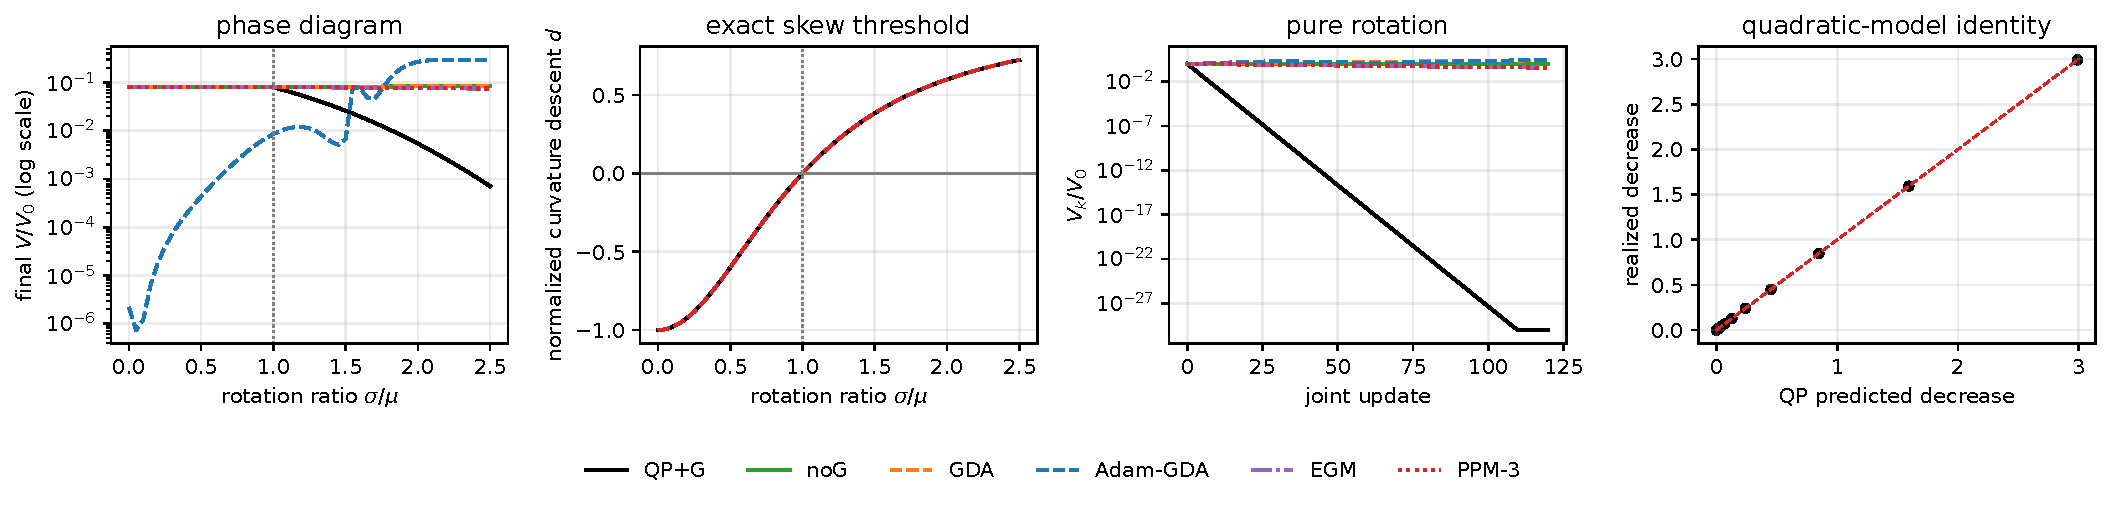
\includegraphics[width=0.925\textwidth]{output/pdf/fig_vi_a_geometry.pdf}
		\caption{Controlled normal-form geometry: normalized field energy, the analytical and computed curvature decrease term $d$, pure-rotation trajectories, and predicted versus realized QP decrease.
			The vertical line marks $\sigma/\mu=1$.}
		\label{fig:controlled_geometry}
	\end{figure*}
	
	\subsection{Tabular Markov games with population oracles}\label{subsec:tabular}
	We retain sequential structure but remove function approximation using one-state
	rock--paper--scissors (RPS), five-state CyclicControl, and eight-state
	FrequencyHopping; each player has three actions and tabular softmax logits.
	RPS is a standard multi-agent RL benchmark \cite{Terry2021PettingZoo}, and
	Appendix~\ref{app:environments} specifies all games.
	For both the tabular and neural population experiments, the QP+G/noG controller
	uses the composite Lyapunov function
	\begin{equation}\label{eq:vic_merit}
		V_{\rm MG}(\bz)
		=0.3\frac{\tfrac12\norm{\bF(\bz)}^{2}}{\kappa_F}
		+\frac{\operatorname{Gap}_{\varepsilon}(\bz)}{\kappa_P},
	\end{equation}
	with normalizers frozen at initialization.
	Population autodifferentiation computes $\bF$ and $\bG=\nabla\bF\,\bF$ while
	each stencil recomputes both regularized BRs.
	The Bellman and Shapley solvers meet numerical tolerance, and
	Eq.~\eqref{eq:performance_bridge} holds at every checkpoint.
	
	Across ten initializations and $100$ joint updates, QP+G attains higher final
	worst-case return and lower mean exploitability than noG in all three games.
	The paired sign tests remain significant after Holm correction across the
	prespecified three-game family \cite{Holm1979}.
	Fig.~\ref{fig:tabular} shows that the same ordering extends to the regularized
	gap and field norm, linking the performance gain to improved saddle-field
	optimization.
	
	\begin{figure*}[!t]
		\centering
		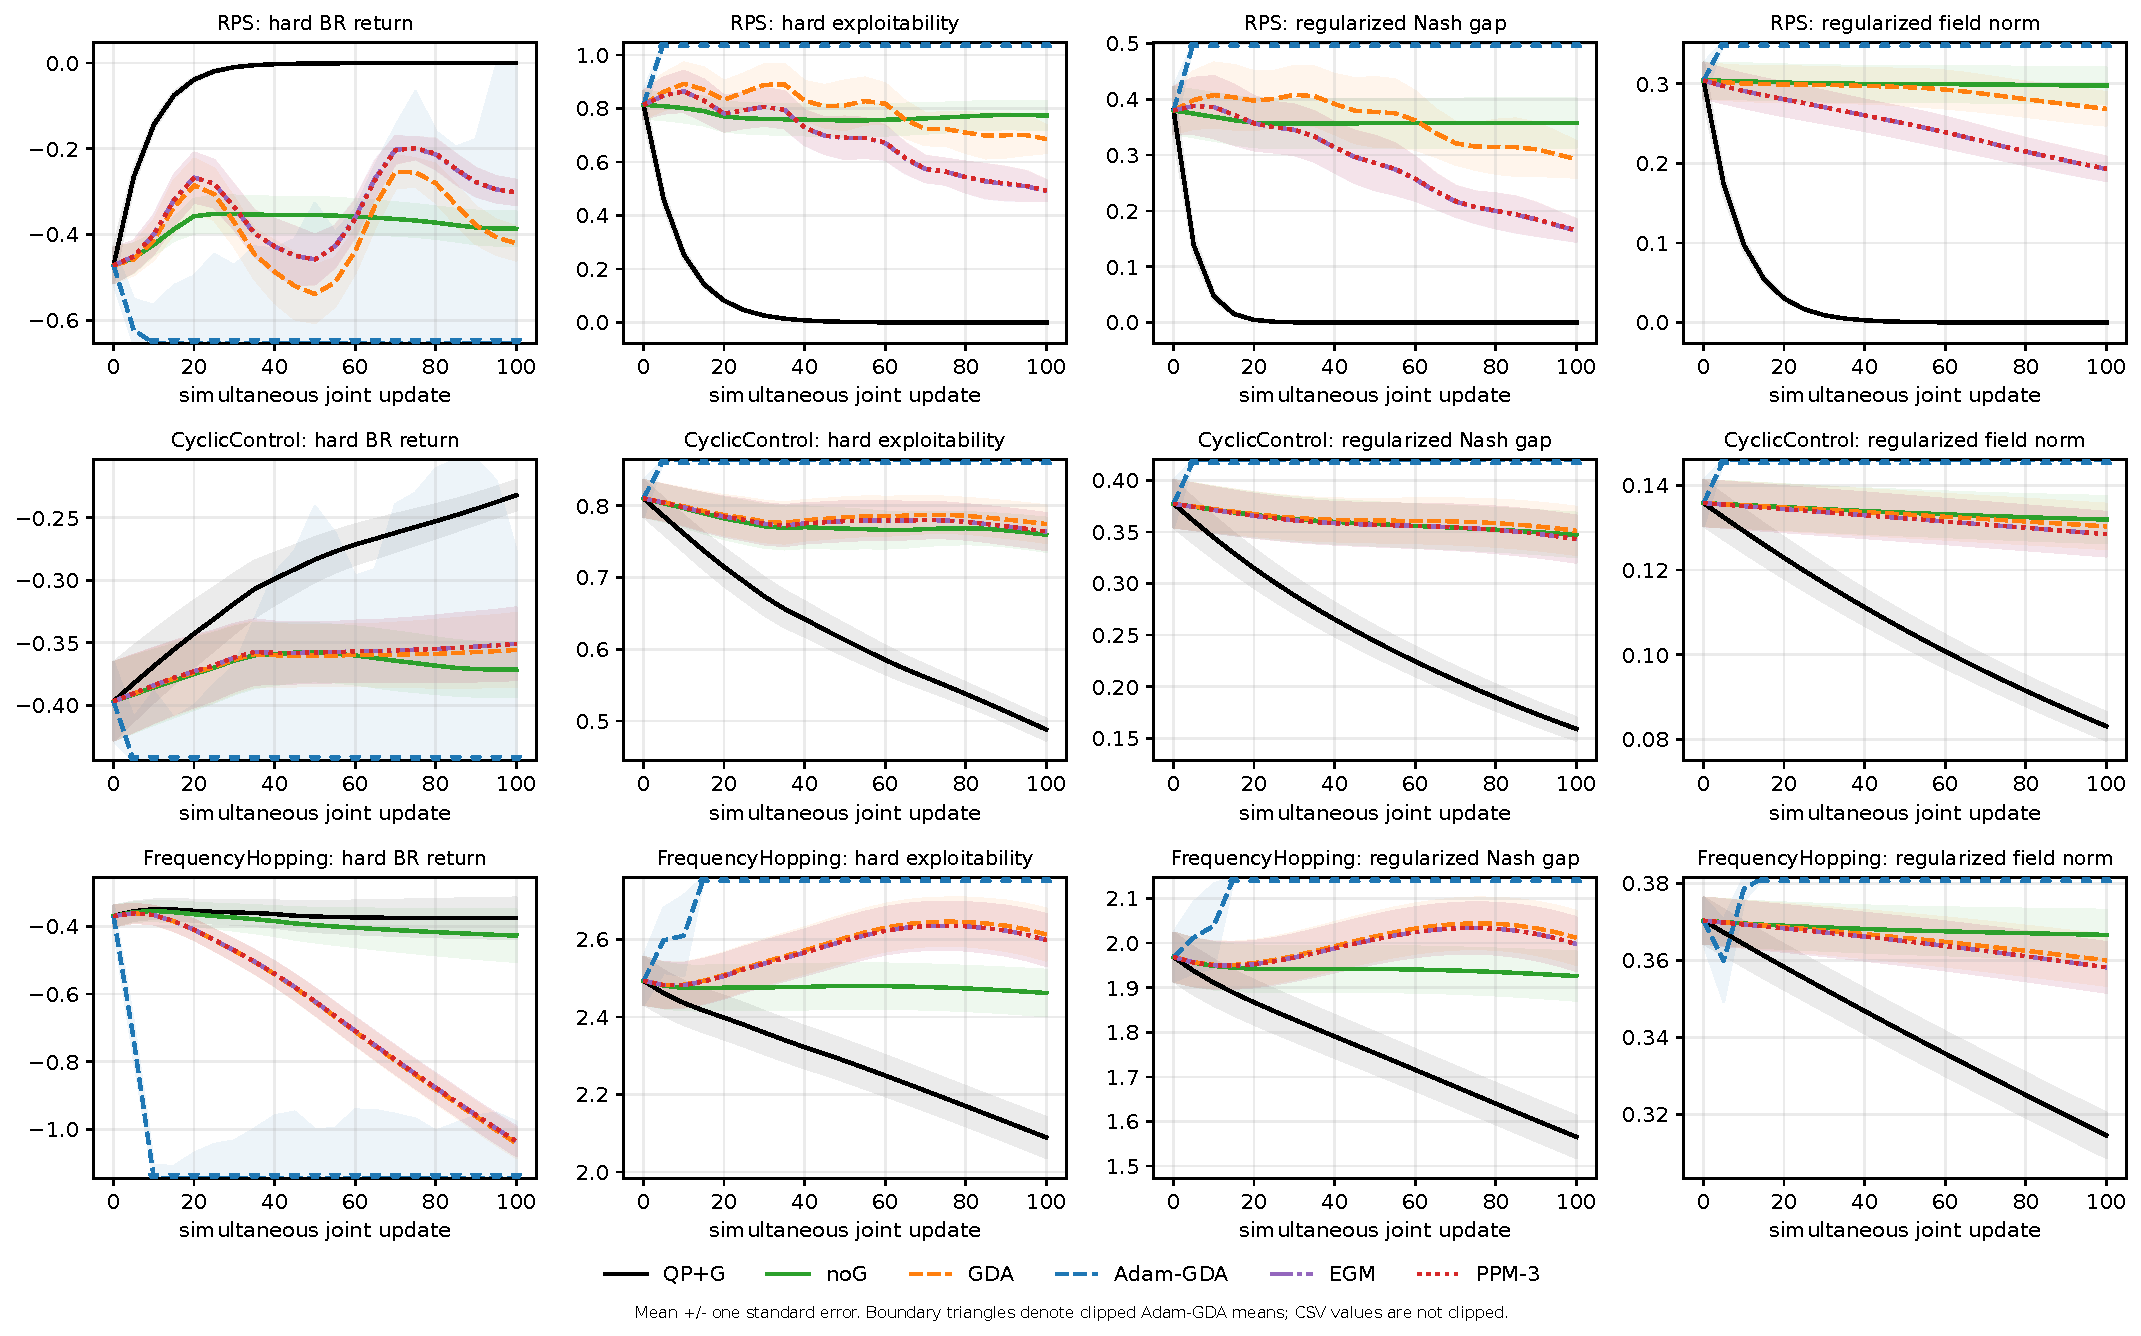
\includegraphics[width=0.875\textwidth]{output/pdf/fig_vi_b_tabular.pdf}
		\caption{Tabular Markov games with population oracles (mean $\pm$ standard error, ten seeds). Columns show worst-case return, exploitability, regularized gap, and field norm; triangles denote clipped Adam-GDA means.}
		\label{fig:tabular}
	\end{figure*}
	
	\subsection{Neural-policy Markov games with population oracles}\label{subsec:neural_mg}
	We train separate $4$--$8$--$3$ tanh--softmax policies for both players,
	forming a $134$-dimensional field on CyclicControl, FrequencyHopping,
	RoutingInterdiction, and SecurityPatrol; Appendix~\ref{app:environments}
	specifies their rewards, transitions, and features.
	
	For each game, $\alpha=0.9$ and $\varepsilon=0.03$; an exact differentiable
	value-system solve yields the population return, $\bF$, and
	$\bG=\nabla\bF\,\bF$.
	Each QP/noG query uses~\eqref{eq:vic_merit} and recomputes both soft BRs at the
	nine central-stencil values.
	For $D\in\{\bF,\bG\}$, the probe is
	$\delta_D=\min\{10^{-2},10^{-3}/\max(\|D\|,10^{-12})\}$; the common spectral
	shift has floor $10^{-8}$.
	The regularized and unregularized best-response solvers meet numerical
	tolerance, and Eq.~\eqref{eq:performance_bridge} holds at every checkpoint.
	
	The evaluation uses ten test seeds and $60$ simultaneous updates, disjoint
	from the screening runs.
	QP+G attains higher final worst-case return and lower mean exploitability
	than noG in all four games, and every paired $95\%$ interval for the
	worst-case-return gain has a positive lower endpoint.
	Fig.~\ref{fig:neural_mg} displays the three unanimous-seed games;
	SecurityPatrol has the same mean ordering.
	On CyclicControl, QP+G reduces mean final exploitability by $79.1\%$, the
	largest relative reduction among the neural-policy games.
	Write $\bF_k\triangleq\bF(\bz_k)$ and $\bG_k\triangleq\bG(\bz_k)$.
	For each QP+G seed--update pair, define the curvature contribution
	$C_k^G=\gamma_k\norm{\bG_k}/
	\max\{\beta_k\norm{\bF_k}+\gamma_k\norm{\bG_k},10^{-15}\}$ and skew ratio
	$R_k=\norm{\bW_k\bF_k}/(\norm{\bS_k\bF_k}+10^{-15})$, where
	$\bS_k=\sym(\nabla\bF(\bz_k))$ and $\bW_k=\skewop(\nabla\bF(\bz_k))$.
	The curvature coordinate activates in every game and contributes
	nontrivially to the update norm.
	The skew ratios for FrequencyHopping and RoutingInterdiction remain near
	unity, consistent with substantial rotational coupling.
	The QP selects the curvature step size from the five estimated terms in
	the local model of the one-step change in $\Vk$.
	
	\begin{figure*}[!t]
		\centering
		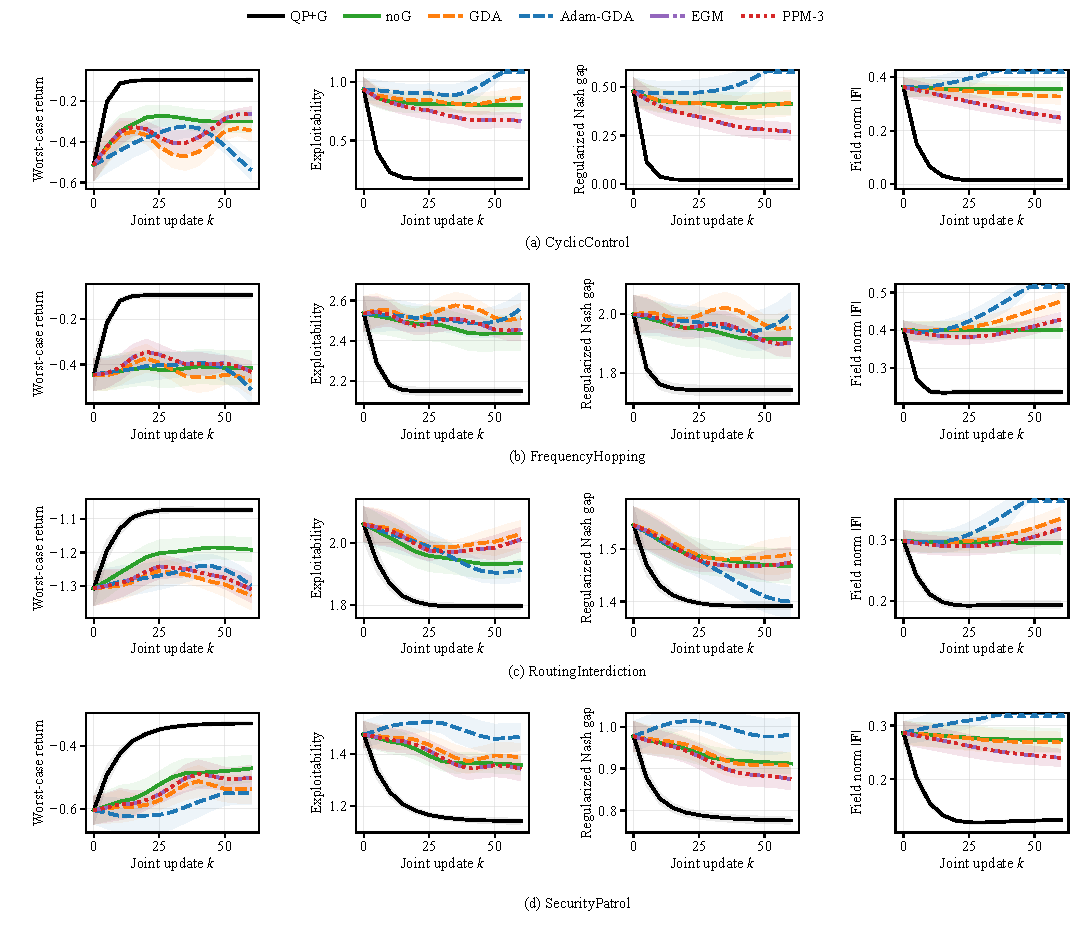
\includegraphics[width=0.875\textwidth]{output/pdf/fig_vi_c_neural.pdf}
		\caption{Neural-policy Markov games for the three unanimous-seed QP+G/noG comparisons (mean $\pm$ standard error, ten seeds). Columns match Fig.~\ref{fig:tabular}; triangles denote clipped Adam-GDA means.}
		\label{fig:neural_mg}
	\end{figure*}
	
	A disjoint screening set selects one global baseline rate from
	$\{0.001,0.003,0.01,0.03\}$: $0.03$ for GDA, EGM, and PPM-3, and $0.001$ for
	Adam-GDA.
	Under this protocol, QP+G achieves the highest mean worst-case return and the
	lowest mean exploitability in all four games.
	
	\subsection{Finite-Trajectory Oracle Validation}\label{subsec:finite_trajectory}
	For CyclicControl, the two $4$--$8$--$3$ policies generate $128$ trajectories
	of horizon $H=16$ ($2048$ transitions) per update.
	We compare the final worst-case return of QP+G and noG after $60$ joint
	updates.
	Detached current-policy probabilities define the behavior distribution, and
	one batch $\mathcal B_k$ evaluates all stencils using unclipped per-decision
	prefix ratios and the infinitely differentiable Monte Carlo estimator (DiCE)
	\cite{Foerster2018DiCE} for causal higher-order score terms.
	Let $\widehat J_{H,k}$ denote the resulting finite-horizon DiCE return
	estimator for batch $\mathcal B_k$.
	We use $\hatF_k=\diag(-\Id,\Id)\nabla\widehat J_{H,k}$ and
	$\hatG_k=\diag(-\Id,\Id)\nabla^2\widehat J_{H,k}\hatF_k$, detaching
	$\hatF_k$ in the Hessian--vector product.
	At stencil point $\bz$, the controller uses
	$\widehat V_k(\bz)=\|\hatF_k(\bz;\mathcal B_k)\|^2/(2\widehat\kappa_F)$,
	with $\widehat\kappa_F$ frozen from an independent initialization batch.
	Training evaluates this field-energy function directly.
	Population quantities are used only for checkpoint evaluation.
	For $\Vk(\bz)=\norm{\bF(\bz)}^2/(2\kappa_F)$,
	Assumption~\ref{ass:oracles} models the field and curvature oracles, while
	dependent same-batch stencil errors enter the local-model estimation-error budget
	of Proposition~\ref{prop:model_approx} and Theorem~\ref{thm:curv_improved}.
	
	On ten held-out test seeds, QP+G improves final worst-case return and reduces
	mean exploitability by $54.0\%$ relative to noG; the paired $95\%$ interval
	for the return gain has a positive lower endpoint.
	QP+G also lowers the final population field norm.
	The curvature coordinate remains active at every update, confirming that the
	sampled-oracle result uses both adaptive directions.
	
	% ============================================================
	\section*{Conclusion}
	% ============================================================
	We introduced an online controller for the field and curvature step sizes in
	stochastic zero-sum Markov-game policy optimization.
	The Jacobian identity states when the curvature direction decreases field
	energy, and the curvature-improvement condition measures its extra decrease in
	the local model of $\Vk$.
	The QP never increases this model relative to feasible field-only and
	fixed-coupling step-size pairs.
	Our finite-time bounds control the average stationarity residual and
	$\E[\Vk]$; the performance corollary then bounds the unregularized Nash gap and
	worst-case-return loss.
	In the tested games, QP+G improves worst-case return and reduces exploitability.
	
	\appendices
	% ============================================================
	
	\section{Proofs}\label{app:proofs}
	\paragraph{Proof of Proposition~\ref{prop:DTA}}\label{app:DTA}
	The GDA identity is immediate.
	On $\bar B(\bz;r)\subset\cD$, let $M_i$ bound $\nabla^i\bF$ for $i=1,2$ and
	$B_F$ bound $\bF$.
	For $s\le\min\{r/B_F,(2M_1)^{-1},1\}$,
	$T_s(\bu)=\bz-s\bF(\bu)$ is a contracting self-map; therefore, its PPM fixed point has
	$\Delta=\bz_+-\bz$ and $\norm{\Delta}\le sB_F$.
	Taylor expansion gives
	$\Delta+s\bF=-s\nabla\bF\,\Delta-s\mathbf r_2$,
	$\norm{\mathbf r_2}\le M_2\norm{\Delta}^2/2$, hence
	$\Delta=-s\bF+s^2\nabla\bF\,\bF+O(s^3)$ uniformly.
	For EGM,
	$\bF(\bz-s\bF)=\bF-s\nabla\bF\,\bF+O(s^2)$ uniformly; multiplication by
	$-s$ gives the same expansion.
	\hfill$\blacksquare$
	
	\paragraph{Proof of Lemma~\ref{lem:decomp}}\label{app:decomp}
	With $\bA=\nabla\bF$ and $\nabla\phi=\bA^\top\bF$,
	$\inner{\nabla\phi}{-\bF}=-\bF^\top\bS\bF$ and
	$\inner{\nabla\phi}{\bG}=\bF^\top\bA^2\bF$.
	Moreover, $\bA^2=\bS^2+\bS\bW+\bW\bS+\bW^2$.
	The cross term vanishes because $\bS\bW+\bW\bS$ is antisymmetric, while
	$\bF^\top\bS^2\bF=\norm{\bS\bF}^2$ and
	$\bF^\top\bW^2\bF=-\norm{\bW\bF}^2$, proving
	\eqref{eq:dphi_F}--\eqref{eq:dphi_G}.
	\hfill$\blacksquare$
	
	\paragraph{Proof of Theorem~\ref{thm:skew_dominance}}\label{app:skew_dominance}
	Eq.~\eqref{eq:dphi_G} proves~\eqref{eq:skew_dominance}.
	For (a), $\bS\bF=0$ gives
	$\inner{\nabla\phi}{\bG}=-\norm{\bW\bF}^{2}<0$ when $\bW\bF\ne0$, whereas
	\eqref{eq:dphi_F} gives $\inner{\nabla\phi}{-\bF}=0$.
	For (b), $\bW=0$ gives
	$\inner{\nabla\phi}{\bG}=\norm{\bS\bF}^{2}\ge0$.
	For (c), normality on the invariant plane gives
	$\bS=\mu\Id$ and $\bW=\sigma J_0$; hence~\eqref{eq:skew_dominance} is equivalent
	to $\lvert\sigma\rvert>\lvert\mu\rvert$.
	\hfill$\blacksquare$
	
	\paragraph{Proof of Corollary~\ref{cor:linear}}\label{app:linear}
	For the linear field $\bF(\bz)=\bA(\bz-\bz^{\star})$, $\nabla\bF(\bz)=\bA$ and $\bG(\bz)=\bA\bF(\bz)=\bA^{2}(\bz-\bz^{\star})$.
	Collinearity $\bG=\lambda\bF$ is equivalent to $\bA\bF=\lambda\bF$.
	If $\bA^\top=-\bA$ and $\bA^2=-\sigma^2\Id$ on the relevant subspace,
	then $\bF=\bA e\perp e$ and $\bG=-\sigma^2e$; hence
	$\bF\perp\bG$, $\inner{\nabla\phi}{-\bF}=0$, and
	$\inner{\nabla\phi}{\bG}=-\sigma^2\norm{\bF}^2
	=-\sigma^4\norm{e}^2$.
	\hfill$\blacksquare$
	
	\paragraph{Proof of Lemma~\ref{lem:Lyap_properties}}\label{app:Lyap_properties}
	Nonnegative summands give $\Vk\ge0$, and $\Vk=0$ forces
	$\cE_F=0$, hence $\bF=0$ because $\lambda_F>0$ and $\bW_V\succ0$.
	Smoothness and the gradient formula follow by composition and the chain rule;
	$\Vk\ge\lambda_F\cE_F/\kappa_F$ with $\Phi=2\cE_F$ gives (d).
	\hfill$\blacksquare$
	
	\paragraph{Proof of Lemma~\ref{lem:drift_taylor}}\label{app:drift_taylor}
	Taylor's theorem along the admissible segment gives the constant, linear, and
	quadratic terms in~\eqref{eq:drift_taylor} and remainder
	$\nabla^3\Vk(\bz_k+\theta\Delta_k)[\Delta_k]^3/6$ for some
	$\theta\in(0,1)$.
	Substitution of~\eqref{eq:drift_terms_def} and
	$\norm{\Delta_k}\le\beta\norm{\hatF_k}+\gamma\norm{\hatG_k}$ gives the bound.
	\hfill$\blacksquare$
	
	\paragraph{Proof of Theorem~\ref{thm:closed_form}}\label{app:closed_form}
	Positive definiteness makes $\hat q_k$ strictly convex.
	Solving
	$\widehat{\bH}_k(\beta,\gamma)^\top=(\hat e_k,\hat d_k)^\top$ gives
	\eqref{eq:unconstrained_pair}; the explicit inverse gives
	\eqref{eq:Delta_hat_interior}.
	If infeasible, the Karush--Kuhn--Tucker (KKT) point lies on an axis, whose
	clipped scalar minimizers are the stated candidates.
	\hfill$\blacksquare$
	
	\paragraph{Proof of Theorem~\ref{thm:dominance}}\label{app:dominance}
	The three comparator sets are subsets of $\R_+^2$, proving dominance by set
	inclusion; their formulas follow by scalar minimization.
	Completing the
	square in~\eqref{eq:Delta_hat_interior} gives
	$\widehat\Delta_k^\star=\hat e_k^2/(2\hat c_k)+
	(\hat b_k\hat e_k+\hat c_k\hat d_k)^2/(2\hat c_k\hat\delta_k)$.
	Subtracting $[\hat e_k]_+^2/(2\hat c_k)$ proves~\eqref{eq:dominance_gap} and
	its equality condition.
	\hfill$\blacksquare$
	
	\paragraph{Proof of Lemma~\ref{lem:pathwise_drift}}\label{app:pathwise_drift}
	Taylor's bound and nonnegative stabilizers give
	$\Vk(\bz_{k+1})-\Vk(\bz_k)\le q_k+\varepsilon_k^{\rm rem}$.
	Applying successively the definitions of $\varepsilon_k^{\rm model}$ and
	$\varepsilon_k^{\rm step}$ gives~\eqref{eq:pathwise_drift}.
	\hfill$\blacksquare$
	
	\paragraph{Proof of Lemma~\ref{lem:residual_budget}}\label{app:residual_budget}
	The step caps and $(a+b)^3\le4(a^3+b^3)$ imply
	$\varepsilon_k^{\rm rem}\le(2M_{3,k}/3)(\beta_{\max}+\gamma_{\max})^3
	(\norm{\hatF_k}^3+\norm{\hatG_k}^3)$.
	Conditional expectation gives
	\eqref{eq:eps_rem_cond}; tower expectation gives uniformity.
	\hfill$\blacksquare$
	
	\paragraph{Proof of Lemma~\ref{lem:local_PL_sufficient}}\label{app:local_PL_sufficient}
	Lemma~\ref{lem:Lyap_properties}(c) and cancellation of the antisymmetric
	quadratic form give a field-energy contribution
	$(\lambda_F/\kappa_F)\bF^\top\sym(\bW_V\nabla\bF)\bF$.
	Applying~\eqref{eq:sym_part_pd}--\eqref{eq:gap_aux_negative_bound} yields
	$\inner{\nabla\Vk}{\bF}\ge
	(\lambda_Fm_F/\kappa_F-\delta_P-\delta_C)\Phi$.
	\hfill$\blacksquare$
	
	\paragraph{Proof of Theorem~\ref{thm:cond_drift}}\label{app:cond_drift}
	Fix $k\ge k_{0}$ and $\bar\beta\ge0$.
	Theorem~\ref{thm:dominance} and
	$[u]_{+}^{2}/(2v)\ge\bar\beta u-\bar\beta^{2}v/2$ give
	$\widehat\Delta_{k}^{\star}\ge\bar\beta\hat e_k-\bar\beta^2\hat c_k/2$.
	Lemma~\ref{lem:pathwise_drift} then gives
	$\Delta\Vk\le-\bar\beta\hat e_k+\bar\beta^2\hat c_k/2+
	\varepsilon_k^{\mathrm{tot}}$.
	Conditional expectation and Assumption~\ref{ass:oracles} yield
	$-\E[\bar\beta\hat e_k\mid\mathscr F_k]\le
	-\bar\beta\inner{\nabla\Vk}{\bF}+\bar\beta G_V\bar b_F$.
	Moreover, $\hat c_k\le H_V\norm{\hatF_k}^2+\rho_{c,k}$ and the three-term
	square bound give
	$\E[\hat c_k\mid\mathscr F_k]\le H_VM_F+\bar\rho_c$.
	Combining proves~\eqref{eq:cond_drift}.
	\hfill$\blacksquare$
	
	\paragraph{Proof of Theorem~\ref{thm:ergodic}}\label{app:ergodic}
	Taking total expectation in~\eqref{eq:cond_drift} and using
	Assumptions~\ref{ass:budget}(c) and~\ref{ass:local}(b) gives
	$\E[\Delta\Vk]\le-\bar\beta\mu_\Phi\E[\Phi(\bz_k)]
	+\mathcal R(\bar\beta)$.
	Sum from $k_0$ to $K-1$, use $\Vk\ge0$, and divide by
	$\bar\beta\mu_\Phi(K-k_0)$.
	\hfill$\blacksquare$
	
	\paragraph{Proof of Theorem~\ref{thm:curv_improved}}\label{app:curv_improved}
	Taylor's bound, model consistency, and accepted-step suboptimality give
	$\Delta\Vk\le-\widehat\Delta_k^{\rm box}
	+\varepsilon_k^{\rm rem}+\varepsilon_k^{\rm model}
	+\varepsilon_k^{\rm step,box}$.
	Since $(\bar\beta,0)$ is box-feasible,
	$\widehat\Delta_k^{F,\rm box}\ge
	\bar\beta\hat e_k-\bar\beta^2\hat c_k/2$.
	Thus $\Delta\Vk\le-\bar\beta e_k+\bar\beta^2(c_k+\rho_{c,k})/2
	-\mathfrak D_{G,k}^{\rm box}+\bar\beta\delta_{e,k}
	+\bar\beta^2\delta_{c,k}/2+\varepsilon_k^{\rm box}$, where
	$\varepsilon_k^{\rm box}$ sums the three residuals above.
	Conditional expectation bounds the first two terms exactly as in
	Theorem~\ref{thm:cond_drift}, while Assumption~\ref{ass:margin} bounds the
	gain term by $-C_G\Phi(\bz_k)+r_{G,k}^{\rm mar}$.
	The stated error,
	margin-residual, and safeguard budgets and Assumption~\ref{ass:local}(b)
	therefore give
	$\E[\Delta\Vk]\le-(\bar\beta\mu_\Phi+C_G)\E[\Phi(\bz_k)]
	+\mathcal R_{\rm box}(\bar\beta)$.
	Telescoping and $\Vk\ge0$ prove~\eqref{eq:curv_improved}.
	\hfill$\blacksquare$
	
	\paragraph{Proof of Corollary~\ref{cor:local}}\label{app:local_cor}
	Taking total expectations in~\eqref{eq:cond_drift} and applying
	Assumptions~\ref{ass:local}(c) and~\ref{ass:budget} gives
	$\E[\Vk(\bz_{k+1})]\le(1-\bar\beta\mu_V)\E[\Vk(\bz_k)]
	+\mathcal R(\bar\beta)$.
	Since
	$q=1-\bar\beta\mu_V\in[0,1)$, iteration yields
	$\E[\Vk(\bz_k)]\le q^{k-k_0}\E[\Vk(\bz_{k_0})]
	+\mathcal R(\bar\beta)\sum_{j\ge0}q^j$; using
	$\sum_{j\ge0}q^j=(\bar\beta\mu_V)^{-1}$ proves the claim.
	\hfill$\blacksquare$
	
	\paragraph{Proof of Proposition~\ref{prop:model_approx}}\label{app:model_approx}
	Subtracting the two quadratic models and applying the five estimation-error
	bounds termwise gives exactly~\eqref{eq:eps_model_bound}.
	\hfill$\blacksquare$
	
	\section{Finite Markov-game environments}\label{app:environments}
	All reported environments have actions $a,b\in\{0,1,2\}$ and initial state
	distribution uniform on $\{0,\ldots,S-1\}$.
	For target map $T(s,a,b)$ and
	noise mass $\xi$, the kernel is
	$P(s'\mid s,a,b)=(1-\xi)\boldsymbol{1}_{\{s'=T(s,a,b)\}}
	+\xi\boldsymbol{1}_{\{s'\ne T(s,a,b)\}}/(S-1)$.
	Let $\varphi_s=2\pi s/S$ and define
	\[
		M
		\triangleq
		\begin{bmatrix}
			0&-1&1\\
			1&0&-1\\
			-1&1&0
		\end{bmatrix}.
	\]
	The one-state RPS game uses reward $M_{ab}$ and a deterministic self-loop;
	the remaining games are:
	\emph{CyclicControl:} $S=5$, $\xi=0.02$,
	$T=(s+1+((a-b)\bmod3))\bmod S$, and
	$r_s(a,b)=(1+0.12\cos\varphi_s)M_{\pi_s(a),\pi_s(b)}$, where
	$\pi_s(j)=(j-s)\bmod3$.
	\emph{FrequencyHopping:} $S=8$, $\xi=0.08$,
	$T=(s+1+a-b)\bmod S$, $q_s(a)=0.25\cos(\varphi_s+2\pi a/3)$, and
	$r_s(a,b)=q_s(a)+0.55$ if $a\ne b$, while
	$r_s(a,a)=q_s(a)-1.10$.
	\emph{RoutingInterdiction:} $S=6$, $\xi=0.10$,
	$T=(s+1+\boldsymbol{1}_{\{a=b\}}+a)\bmod S$,
	$c_s(a)=1+0.20\sin(\varphi_s+2\pi a/3)$, and
	$r_s(a,b)=c_s(a)-0.55-1.35\boldsymbol{1}_{\{a=b\}}-0.15\boldsymbol{1}_{\{a\ne b\}}$.
	\emph{SecurityPatrol:} $S=8$, $\xi=0.08$,
	$T=(s+1+b+\boldsymbol{1}_{\{a\ne b\}})\bmod S$,
	$v_s(b)=0.8+0.25\cos(\varphi_s+2\pi b/3)$, and
	$r_s(a,b)=v_s(b)$ if $a=b$, while $r_s(a,b)=-0.55v_s(b)$ otherwise.
	Neural policies use $x_s=(\sin\varphi_s,\cos\varphi_s,u_s,1)$, where, in the
	order above, $u_s$ is $s/(S-1)$, the range of $q_s$, the standard deviation of
	$c_s$, and the mean of $v_s$.
	The last two are grid-constant architecture
	coordinates; state variation is encoded by $(\sin\varphi_s,\cos\varphi_s)$.
	\bibliographystyle{IEEEtran}
	\bibliography{refs}
\end{document}
